\documentclass[conference]{IEEEtran}

% --- REQUIRED PACKAGES ---
\usepackage{amsmath}
\usepackage{amssymb}
\usepackage{graphicx}
\usepackage{booktabs}
\usepackage{url}
\usepackage{bm}
\usepackage{cite}

\begin{document}

% --- TITLE & AUTHOR BLOCK ---
\title{Speed-Invariant Continuous Road Roughness (IRI) Estimation via Physics-Informed Smartphone Sensing and Soft-Body Simulation Ground Truth}

\author{
\IEEEauthorblockN{Nishkarsh Singhal}
\IEEEauthorblockA{\textit{Department of Electronics and Communication Engineering} \\
\textit{Faculty of Technology, University of Delhi}\\
New Delhi, India}
}

\maketitle

% --- ABSTRACT ---
\begin{abstract}
Continuous monitoring of urban pavement roughness is critical for infrastructure preservation, yet Class 1 laser profilometers remain cost-prohibitive ($>\$50,000$ per vehicle). While crowdsourced smartphone inertial sensing offers a scalable alternative, existing models suffer from single-vehicle empirical overfitting and speed-dependent signal distortion ($a_z \propto v^2$). In this paper, we present a speed-invariant, vehicle-agnostic International Roughness Index (IRI) estimation architecture trained via a Sim-to-Real (Sim2Real) soft-body physics pipeline. Leveraging BeamNG.tech across three distinct vehicle classes and urban/rural environments, we formulate a Curvature-Adaptive Mesh Tessellation Correction to resolve artificial 3D polygon-facet slope oscillations and generate standardized quarter-car ground truth. The resulting synthetic corpus trains a lightweight Dual-Branch Depthwise-Separable 1D-CNN incorporating kinetic normalization, 2-D inverse-frequency sampling, Asymmetric Huber Loss, and Post-Training Isotonic Calibration (PICA). On a multi-vehicle validation benchmark, our model achieves a Mean Absolute Error of $1.642\,\text{m/km}$ ($R^2 = 0.493$), outperforming gradient-boosted trees by 19.1\% and sequential recurrent networks by 30.9\%. Under AASHTO R 56 standards, the model achieves 77.9\% compliance at municipal screening thresholds ($\pm 1.5\,\text{m/km}$). Furthermore, zero-shot evaluation on the real-world crowdsourced PVS dataset ($693\,\text{km}$) confirms cross-domain transferability across heterogeneous speeds and road surfaces, establishing a deployable edge-inference engine for participatory road monitoring.
\end{abstract}

% --- KEYWORDS ---
\begin{IEEEkeywords}
International Roughness Index (IRI), participatory sensing, smartphone IMU, Sim-to-Real transfer, BeamNG.tech simulation, curvature-adaptive mesh correction, depthwise-separable 1D-CNN, asymmetric Huber loss, isotonic calibration, speed invariance, AASHTO R 56 benchmarking, crowdsourced road monitoring.
\end{IEEEkeywords}

% ==========================================
% I. INTRODUCTION
% ==========================================
\section{Introduction}

\subsection{The Global Pavement Monitoring Gap and Economic Impact}
Road pavement infrastructure represents one of the most capital-intensive physical assets managed by municipal governments worldwide. In extensive national networks such as India's 6.3 million-kilometer roadway system~\cite{1}, routine structural condition assessment on secondary and tertiary roads occurs infrequently—often spanning intervals of three to five years~\cite{1}. Globally, pavement deterioration inflicts severe economic burdens: the World Bank estimates that poor road conditions cost vehicle owners more than \$500 billion annually through accelerated tire wear, drivetrain damage, fuel overconsumption, and road accident externalities~\cite{2}.

The internationally established standardized metric for quantifying pavement roughness is the International Roughness Index (IRI), standardized under ISO 8608 and ASTM E1926~\cite{3}. IRI measures the cumulative vertical suspension displacement of a standardized World Bank Quarter-Car (Golden Car) traversing a road profile at a reference velocity of $80\,\text{km/h}$ ($22.22\,\text{m/s}$), expressed in meters per kilometer ($\text{m/km}$). Professional municipal surveys rely on Inertial Profiling Systems (IPS)—specialized vehicles equipped with high-precision optical laser displacement sensors and inertial navigation systems. While Class 1 laser profilometers achieve sub-millimeter vertical precision ($\pm 0.1\,\text{m/km}$), their initial capital expenditure ($>\$50,000\text{--}\$200,000$ USD per vehicle) and recurring calibration overhead render city-scale continuous monitoring economically intractable. Consequently, defects progress undetected between periodic surveys, motivating the urgent need for a ubiquitous, scalable, low-cost pavement monitoring layer.

\subsection{Smartphone Participatory Sensing and Empirical Overfitting Limitations}
With over 6.8 billion active devices globally, modern smartphones equipped with multi-axis MEMS Inertial Measurement Units (IMUs) and GNSS receivers present a transformative opportunity for participatory or opportunistic sensing~\cite{4}. Since the foundational Nericell framework~\cite{5}, extensive research has explored converting passenger vehicles into crowdsourced road surface probes~\cite{6,7,8}.

However, a critical methodological limitation pervades the existing experimental literature: \textbf{the empirical ground-truth acquisition bottleneck}. The vast majority of published studies collect empirical IMU training datasets from a single test vehicle (or at most two homogeneous vehicles) driven over restricted, localized road segments~\cite{6,7}. Even when studies incorporate co-registered laser profilometer measurements alongside cabin smartphone sensors~\cite{6}, the resulting predictive models remain fundamentally bound to the host vehicle's mechanical transfer function $\mathcal{T}_{\text{veh}}$. Because passenger vehicle suspensions act as complex, non-linear mechanical filters—differing drastically between a stiff utility vehicle and a soft-sprung sedan—an empirical model trained on one cabin configuration exhibits severe systematic bias when deployed in another. Furthermore, empirical field collection over narrow road stretches frequently omits critical surface anomalies and terrain classifications, preventing models from generalizing to complex municipal road networks.

\subsection{Two Fundamental Scientific Challenges}
Designing a genuinely generalizable, speed-invariant smartphone IRI estimator requires overcoming two unsolved physical and computational challenges:

\subsubsection{Challenge 1 — The Sim-to-Real Ground-Truth Acquisition Bottleneck}
Obtaining synchronized, centimeter-accurate elevation profile ground truth ($h(x)$) paired with cabin IMU telemetry across diverse vehicle suspension stiffnesses, payload masses, and arbitrary speed profiles is logistically intractable in the physical world. While physics simulators have been successfully adopted in autonomous driving perception research, simulating structural pavement roughness requires a soft-body physics engine capable of resolving tire-contact enveloping, damper hysteresis, and chassis flex. Furthermore, 3D polygonal mesh simulators introduce a subtle geometric artifact: on curved roads or sloped ramps, adjacent planar polygon facets meet at dihedral angles, creating artificial high-frequency slope oscillations that severely distort quarter-car IRI calculations.

\subsubsection{Challenge 2 — Velocity-Squared Dynamic Coupling and the Staircase Artifact}
Standard smartphone IMUs sample acceleration in the temporal domain ($t$), whereas pavement roughness is a spatial geometric property ($\lambda$). The relationship is governed by vehicle velocity $v$, where a spatial undulation of wavelength $\lambda$ excites the suspension at temporal frequency $f = v/\lambda$. Simultaneously, kinetic energy transfer scales the amplitude of vertical acceleration quadratically ($a_z \propto v^2$). When standard time-domain convolutional or recurrent neural networks process unscaled IMU time series, any change in vehicle speed—such as accelerating from a traffic signal or decelerating for congestion—induces severe step-change discontinuities in predicted roughness (the ``staircase artifact'') on physically uniform pavement.

\subsection{Summary of Contributions}
To address these limitations, this paper presents a complete Sim-to-Real (Sim2Real) continuous IRI estimation architecture designed for deployment on edge consumer smartphones within a crowdsourced participatory network. Our core technical contributions are:

\begin{enumerate}
    \item \textbf{Curvature-Adaptive Mesh Tessellation Correction for Sim2Real Ground Truth:} We identify and mathematically resolve artificial polygon-facet jitter in 3D vehicular simulators, formulating a curvature-adaptive smoothing algorithm that dynamically separates horizontal/vertical slope bending ($\kappa$) from true vertical roughness. This allows high-fidelity IRI ground truth to be generated across all simulated road geometries.
    \item \textbf{Multi-Vehicle, Multi-Environment Sim2Real Training Corpus:} We exploit the BeamNG.tech soft-body physics engine to generate synchronized LiDAR elevation profiles and dashboard IMU traces across 3 distinct vehicle classes (Roamer SUV, Vivace Hatchback, Sunburst Sedan) and 3 customized terrain environments (East Coast USA, West Coast USA, Automation Test Track) under highly variable speed profiles, decoupling speed variation from reference $80\,\text{km/h}$ IRI labels.
    \item \textbf{Speed-Invariant Dual-Branch 1D-CNN with Asymmetric Huber Loss and PICA:} We propose a lightweight dual-branch network combining depthwise-separable 1D convolutions over $100\,\text{m}$ spatial windows with inverse quadratic kinetic normalization $(22.22/v_{\text{safe}})^2$ and 2-D inverse-frequency joint histogram sampling. An Asymmetric Huber Loss ($\delta=1.0$, 4:1 over-prediction penalty) and Post-Training Isotonic Regression Calibration (PICA) correct boundary shrinkage and asymmetric severity bias.
    \item \textbf{Comprehensive Standards Compliance and Zero-Shot Real-World Validation:} We benchmark the proposed architecture against 10 ML/DL baselines and formal AASHTO Practice R 56 screening thresholds. Furthermore, we validate zero-shot domain transfer on the public PVS real-world crowdsourced dataset ($693\,\text{km}$ across 9 trips), revealing and physically explaining the cobblestone versus unpaved dirt road biomechanical inversion.
\end{enumerate}

The remainder of this paper is organized as follows: Section~II reviews related work. Section~III details the synthetic ground-truth acquisition and IRI computation methodology. Section~IV presents the speed-invariant deep learning architecture. Section~V discusses empirical evaluation and benchmarking results. Section~VI concludes with a municipal deployment roadmap.

% ==========================================
% II. RELATED WORK
% ==========================================
\section{Related Work}

\subsection{Standardized Pavement Roughness Measurement and Municipal Practices}
The international standard for quantifying road surface roughness is the International Roughness Index (IRI), established by the World Bank in 1986~\cite{3} and standardized under ASTM E1926 and ISO 8608. IRI represents the accumulated vertical suspension stroke of a mathematical quarter-car representation—the World Bank Golden Car—traversing a longitudinal elevation profile at a reference velocity of $80\,\text{km/h}$, expressed in $\text{m/km}$. Professional civil engineering evaluation relies on Inertial Profiling Systems (IPS): vehicles equipped with laser displacement sensors, optical encoders, and high-precision inertial navigation platforms. Under American Association of State Highway and Transportation Officials (AASHTO) Standard Practice R 56~\cite{aashto_r56}, Class 1 inertial profilometers achieve sub-millimeter precision ($\pm 0.1\text{--}0.25\,\text{m/km}$). However, their capital procurement cost ($>\$50,000\text{--}\$200,000$ USD per vehicle) and operational complexity restrict routine municipal surveys to primary arterial corridors, leaving residential, secondary, and rural networks unmonitored for multi-year cycles.

\subsection{Smartphone-Based Participatory Sensing and Empirical Field Limitations}
To bridge the municipal monitoring gap, researchers have increasingly investigated opportunistic or participatory sensing using consumer smartphones~\cite{4,5}. Early frameworks relied on threshold heuristics applied to vertical accelerometer ($a_z$) peaks to flag discrete anomalies such as potholes or speed breakers~\cite{11,14}. Subsequent work applied statistical machine learning ensembles—including Random Forests, Support Vector Machines, and Gradient Boosted Decision Trees (XGBoost, LightGBM)—to statistical time-domain features extracted from cabin IMU traces~\cite{6,7}. More recently, deep learning architectures such as 1D Convolutional Neural Networks (CNNs) and Long Short-Term Memory (LSTM) networks have been adopted to regress continuous IRI values from multi-axis inertial time series~\cite{8}.

Despite substantial algorithmic progress, existing smartphone-based IRI estimation literature suffers from a pervasive methodological confound: \textbf{empirical field-data overfitting}. In high-quality recent experimental studies where researchers mount a professional Class 1 laser profilometer alongside cabin smartphone IMUs on a physical test vehicle to obtain co-registered $(a_z(t), \text{IRI})$ training pairs~\cite{6,7}, data collection is almost universally restricted to a single host vehicle traversing a localized set of road categories. Formally, the cabin vertical acceleration $a_z(t)$ observed by a smartphone is related to the true pavement elevation profile $h(x)$ via an unknown, highly non-linear suspension transfer function:
\begin{equation}
a_z(t) = \mathcal{T}_{\text{veh}}\bigl(h(x(t)),\, \dot{x}(t),\, m_{\text{load}},\, c_s,\, k_s\right) + \epsilon(t)
\end{equation}
where $\dot{x}(t)$ is traversal velocity, $m_{\text{load}}$ is cabin payload mass, and $c_s, k_s$ represent damping and spring stiffness coefficients. When an empirical regression model is trained on data collected from a single vehicle (e.g., a mid-size passenger sedan), the neural network or tree ensemble inadvertently learns the inverse transfer function $\mathcal{T}_{\text{veh}}^{-1}$ specific to that chassis configuration. Consequently, when deployed in a vehicle with a stiffer suspension profile (e.g., a utility SUV or light truck), the model exhibits systematic bias, misclassifying smooth pavement as rough due to higher transmitted acceleration amplitudes. Furthermore, empirical collection over limited road stretches frequently fails to represent diverse pavement anomalies and surface materials. Finally, because IMU sensors sample in the temporal domain ($f = v/\lambda$), models trained without spatial kinetic normalization suffer from velocity-induced ``staircase artifacts'' when vehicles accelerate or brake over uniform pavement~\cite{6,8}.

\subsection{Sim-to-Real Transfer and 3D Mesh Tessellation Artifacts}
To overcome the empirical data scarcity bottleneck and achieve vehicle-agnostic generalization, synthetic physics simulation offers a deterministic vehicular laboratory. While simplified rigid-body simulators provide basic kinematic traces, they fail to model pneumatic tire contact-patch enveloping, damper hysteresis, or chassis flex. In contrast, soft-body physics engines such as BeamNG.tech model vehicles as fully deformable finite-element meshes, simulating tire-surface frictional contact and multi-link suspension dynamics from first principles~\cite{15}. While Sim-to-Real (Sim2Real) transfer has become standard practice in autonomous driving perception and ADAS control verification, our work is the first to establish a rigorous Sim2Real zero-shot transfer pipeline for continuous pavement roughness (IRI) regression.

However, exploiting 3D vehicular simulators for sub-centimeter elevation profiling introduces a non-trivial computational geometry challenge: \textbf{polygon-mesh tessellation artifacts}. In 3D simulation engines, road surfaces are rendered from planar polygon facets. On flat horizontal terrain, adjacent facets are coplanar; however, on road segments with vertical curvature—such as highway flyovers, elevated ramps, or grade transitions—adjacent planar facets meet at small dihedral angles. When a virtual vehicle traverses these dihedral edges, the sharp geometric transitions induce artificial high-frequency vertical acceleration spikes ($\pm 0.3\,\text{m/m}$ slope jitter) concentrated precisely in the $1\text{--}3\,\text{m}$ spatial wavelength band. Left uncorrected, feeding these raw simulation profiles into the Golden Car quarter-car model inflates calculated IRI to $15\text{--}16\,\text{m/km}$ on sloped ramps that are geometrically smooth by design. Prior literature utilizing simulated vehicle traces has not identified or corrected this mesh rendering artifact. Our proposed Curvature-Adaptive Mesh Tessellation Correction directly addresses this challenge.

% ==========================================
% III. METHODOLOGY: SYNTHETIC GROUND TRUTH & IRI PIPELINE
% ==========================================
\section{Methodology: Synthetic Ground Truth Acquisition and Continuous IRI Pipeline}

\subsection{Sim-to-Real Synthetic Data Acquisition in BeamNG.tech}

\subsubsection{The Deterministic Soft-Body Physics Laboratory}
To eliminate empirical overfitting and obtain zero-noise co-registered ground truth, we utilize BeamNG.tech (v0.38.3.0) as a deterministic vehicular physics laboratory. Unlike rigid-body simulators, BeamNG.tech models vehicles as deformable finite-element soft-body structures where every structural node participates in physical load transfer. Tire contact patches, hydraulic damper hysteresis, and multi-link suspension geometries are modeled from first principles, providing sufficient fidelity for automotive ADAS validation~\cite{15}.

\begin{figure}[t]
\centering
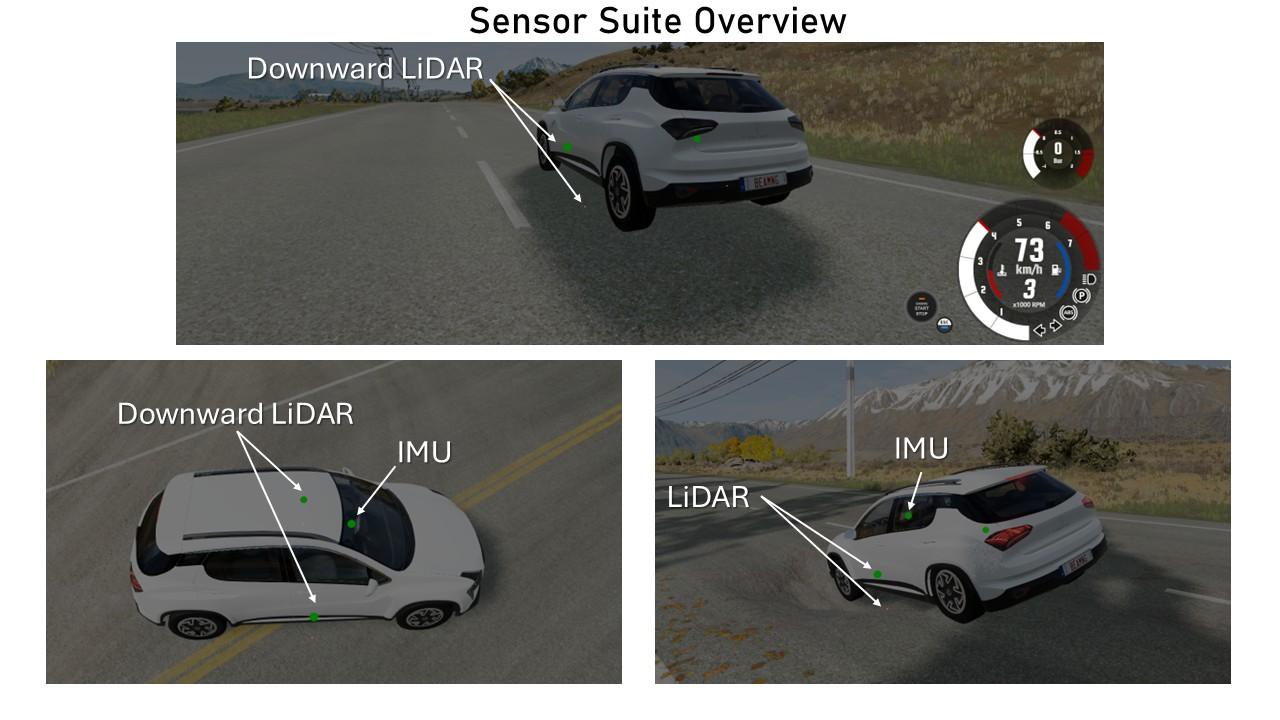
\includegraphics[width=\linewidth]{images/beamNG_sensor_placement.jpg}
\caption{Virtual sensor placement and spatial sampling architecture within the BeamNG.tech simulation environment. Synchronized data acquisition combines dual downward-facing LiDAR sensors mounted at left and right wheel tracks ($\pm 0.85\,\text{m}$ lateral offset) for road elevation profiling $h(x)$ alongside a dashboard-mounted virtual \texttt{AdvancedIMU} recording 3-axis linear acceleration and angular velocity.}
\label{fig:sensor_placement}
\end{figure}

Within the simulation, we establish synchronized oracle access to both true pavement surface elevation and cabin inertial dynamics (Figure~\ref{fig:sensor_placement}). We deploy three parallel daemon threads communicating with the simulation engine via thread-safe shared memory:
\begin{enumerate}
    \item \textbf{LiDAR Elevation Profiler (\texttt{LidarWorker}):} Dual narrow-beam downward-facing LiDAR sensors are mounted at left and right wheel tracks ($\pm 0.85\,\text{m}$ lateral offset relative to vehicle centerline), polling surface elevation at $f_{\text{IRI}} = 100\,\text{Hz}$ to record instantaneous left and right elevation traces $h_L(t)$ and $h_R(t)$ alongside 2D geographic coordinates $(p_x, p_y)$ into \texttt{iri\_sensor\_data.csv}.
    \item \textbf{Dashboard Smartphone IMU Probe (\texttt{ImuStateWorker}):} A virtual \texttt{AdvancedIMU} sensor is mounted inside the vehicle cabin at the dashboard center—precisely replicating an edge smartphone inside a dashboard cradle. The probe records 3-axis linear acceleration, 3-axis angular velocity, and instantaneous vehicle velocity at $f_{\text{IMU}} = 100\,\text{Hz}$ into \texttt{imu\_speed\_data.csv}.
    \item \textbf{Visual Context (\texttt{CameraWorker}):} A forward-facing dashcam records visual imagery at $20\,\text{Hz}$ for contextual alignment.
\end{enumerate}

To ensure seamless transfer to real-world edge devices, we perform explicit coordinate re-mapping within \texttt{ImuStateWorker} to convert BeamNG's native world coordinate axes into standard right-handed smartphone IMU conventions (Table~\ref{tab:imu_mapping}).

\begin{table}[t]
\centering
\caption{Coordinate Re-Mapping from BeamNG to Physical Smartphone Frame}
\label{tab:imu_mapping}
\resizebox{\columnwidth}{!}{
\begin{tabular}{lll}
\toprule
\textbf{BeamNG Raw Channel} & \textbf{Physical Smartphone Axis} & \textbf{Mapped Key} \\
\midrule
\texttt{acc[2]} (Lateral, Y-world) & Left-Right Acceleration & \texttt{ax} \\
\texttt{acc[0]} (Longitudinal, X-world) & Front-Back Acceleration & \texttt{ay} \\
\texttt{acc[1]} (Vertical, Z-world) & Up-Down Acceleration & \texttt{az} \\
\texttt{gyro[2]} (Pitch rate) & Pitch Angular Rate & \texttt{wx} \\
\texttt{gyro[0]} (Roll rate) & Roll Angular Rate & \texttt{wy} \\
\texttt{gyro[1]} (Yaw rate) & Yaw Angular Rate & \texttt{wz} \\
\bottomrule
\end{tabular}
}
\end{table}

\subsubsection{Multi-Vehicle and Multi-Environment Selection}
While BeamNG.tech provides a vast catalog of vehicular models and terrains, we specifically selected three representative vehicle platforms spanning the primary mechanical suspension classes present in real-world traffic:
\begin{itemize}
    \item \textbf{Roamer (Stiff SUV / Light Truck):} Body-on-frame multi-utility vehicle with high unsprung mass and stiff suspension damping.
    \item \textbf{Sunburst2 (Mid-Size Sedan):} Monocoque passenger sedan with balanced spring and damper characteristics.
    \item \textbf{Vivace (Hatchback):} Compact passenger hatchback with compliant, soft-sprung suspension tuning.
\end{itemize}

To represent diverse urban and rural infrastructure, we customized three simulation environments by injecting structural surface defects, potholes, and irregular patches:
\begin{itemize}
    \item \textbf{East Coast USA:} Countryside and hilly roadways with unpaved dirt stretches and undulating grades.
    \item \textbf{West Coast USA:} Metropolitan urban arterials, highway interchanges, and high-speed expressways.
    \item \textbf{Automation Test Track:} A dedicated controlled circuit containing varied road surface textures and calibrated obstacles, utilized primarily for model verification and validation.
\end{itemize}

\subsubsection{Variable-Speed Data Collection vs. Reference IRI Calculation}
A critical methodological design decision concerns traversal velocity. Simulating vehicles driving at a constant reference velocity of $80\,\text{km/h}$ would introduce severe speed overfitting: the deep learning model would memorize 80\,km/h spectral frequencies rather than generalizing to real-world traffic where speeds vary continuously. Therefore, data collection runs were executed under \textbf{highly variable speed profiles}, capturing rash high-speed driving on open stretches, careful slow crawling ($10\text{--}25\,\text{km/h}$) in congested sections, and moderate mixed-traffic transitions.

Crucially, this speed variation affects only the \textbf{cabin IMU feature matrix}. IRI is a spatial geometric property of the pavement $h(x)$, invariant to the velocity of any physical survey vehicle. After spatial resampling of the elevation profiles $h_L(l)$ and $h_R(l)$, the Golden Car quarter-car state-space model is simulated over the spatial profile at the standardized reference velocity of $v_{\text{ref}} = 80\,\text{km/h}$ ($22.22\,\text{m/s}$), ensuring that the ground-truth IRI label strictly adheres to ISO 8608 regardless of the variable collection speed.

\subsection{The Five-Stage Continuous IRI Ground-Truth Pipeline}
Synchronized IMU and elevation traces are processed through a five-stage pipeline to establish calibrated continuous IRI ground truth (\texttt{readings\_2.csv}).

\subsubsection{Stage 1 — Spatial Resampling}
Cumulative horizontal 2D distance $l_k$ along the road center spline is computed from successive planar coordinate deltas:
\begin{equation}
l_k = \sum_{i=1}^{k} \sqrt{(\Delta p_{x,i})^2 + (\Delta p_{y,i})^2}
\end{equation}
Left and right elevation traces $h_L(l)$ and $h_R(l)$ are linearly interpolated onto a uniform spatial grid with interval $\Delta x = 0.25\,\text{m}$, meeting ASTM E1926 canonical sampling standards.

\subsubsection{Stage 2 — Curvature-Adaptive Mesh Tessellation Correction}
As established in Section~II, planar polygon facets meeting at dihedral angles on sloped or curved roads induce severe artificial slope jitter ($\pm 0.3\,\text{m/m}$) concentrated in the $1\text{--}3\,\text{m}$ spatial wavelength band (Figure~\ref{fig:mesh_psd}). Uncorrected, this rendering artifact inflates raw IRI to $15\text{--}16\,\text{m/km}$ on smooth ramps.

\begin{figure*}[t]
\centering
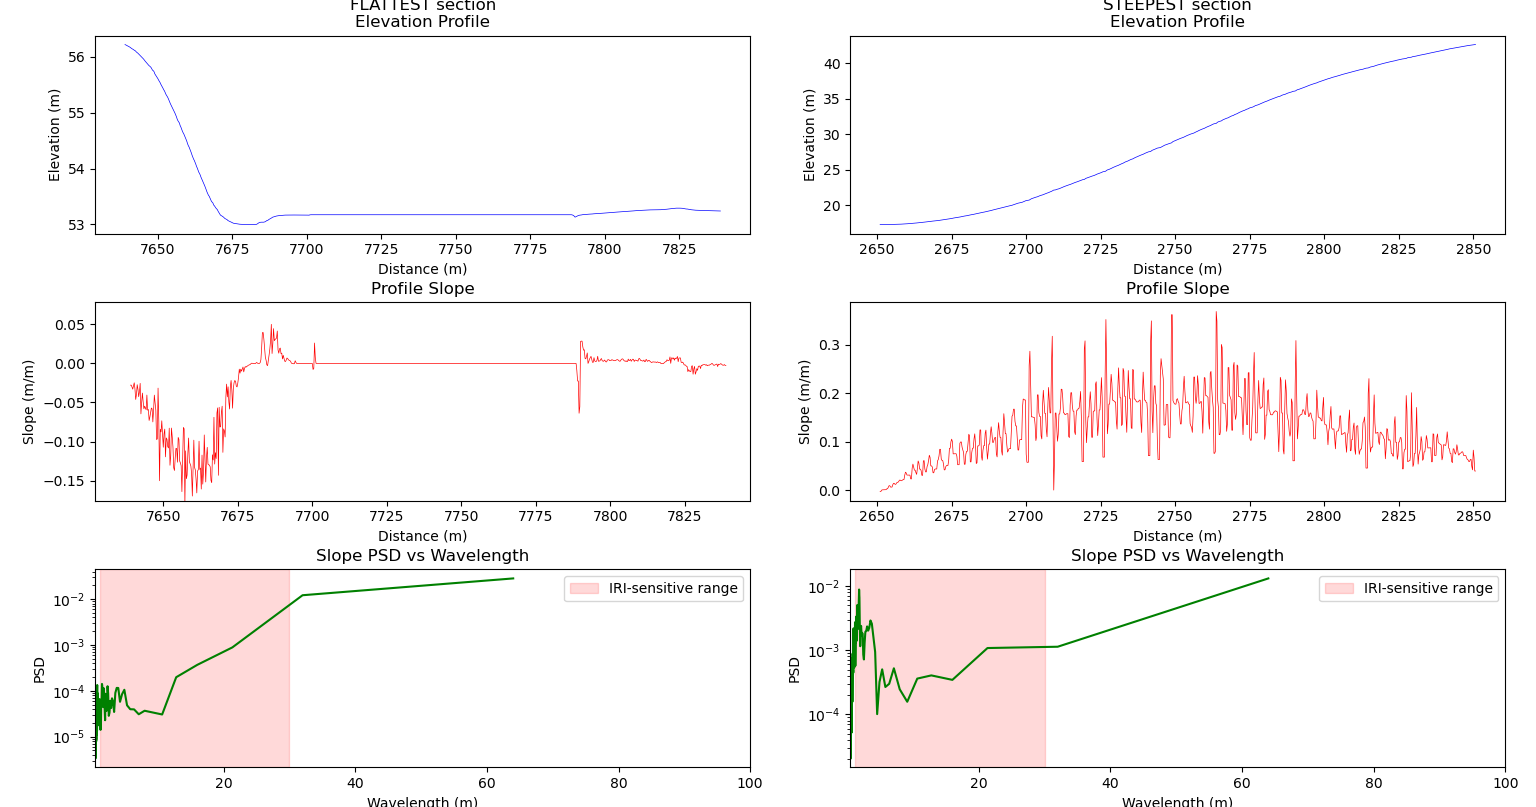
\includegraphics[width=\textwidth]{images/mesh_poygon_analysis.png}
\caption{Empirical Power Spectral Density (PSD) analysis of polygon-mesh tessellation jitter in BeamNG.tech simulation data. Left column: flat road section exhibiting smooth elevation, near-zero slope noise, and negligible PSD energy in the IRI-sensitive band ($1\text{--}30\,\text{m}$). Right column: sloped section exhibiting severe high-frequency slope oscillations ($\pm 0.3\,\text{m/m}$) concentrated entirely in the $1\text{--}10\,\text{m}$ IRI-sensitive band due to dihedral polygon facet edges.}
\label{fig:mesh_psd}
\end{figure*}

\begin{figure*}[t]
\centering
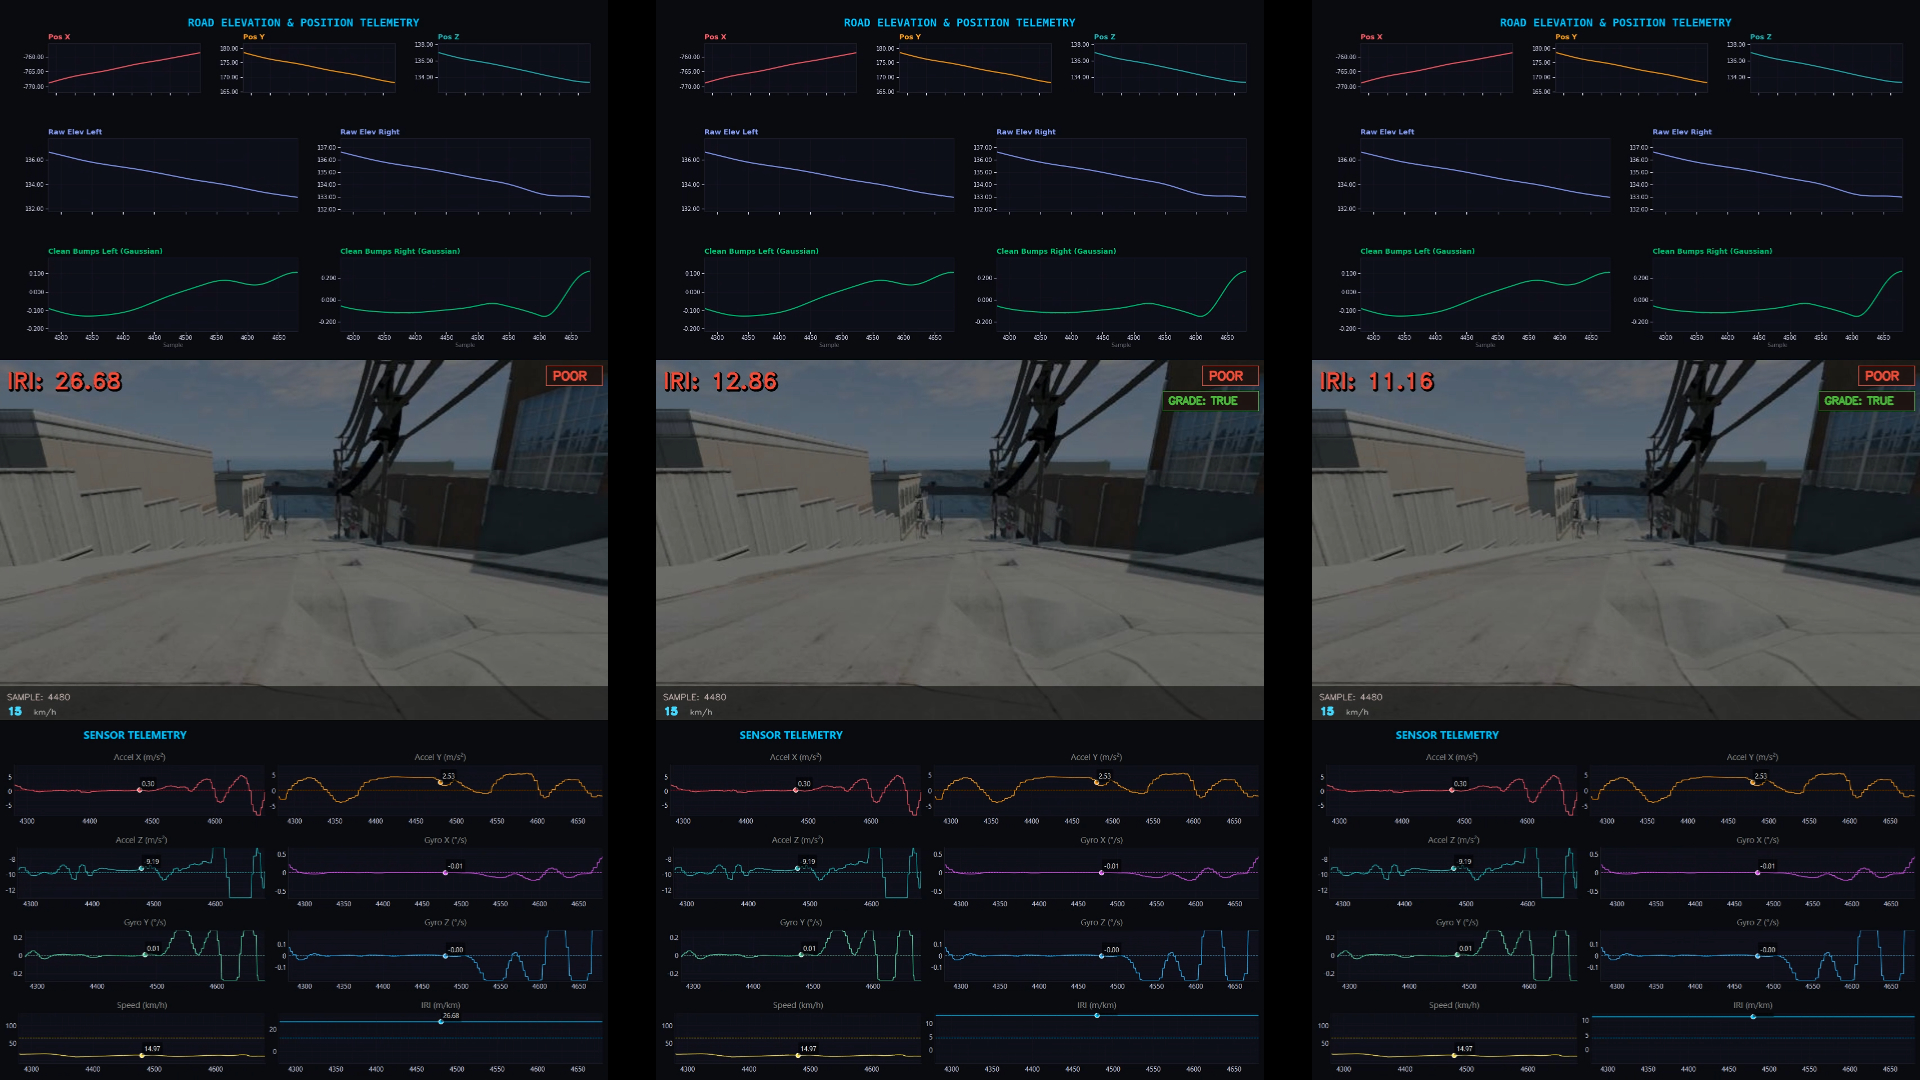
\includegraphics[width=0.48\textwidth]{images/CAP_bad_slope.jpg}
\hfill
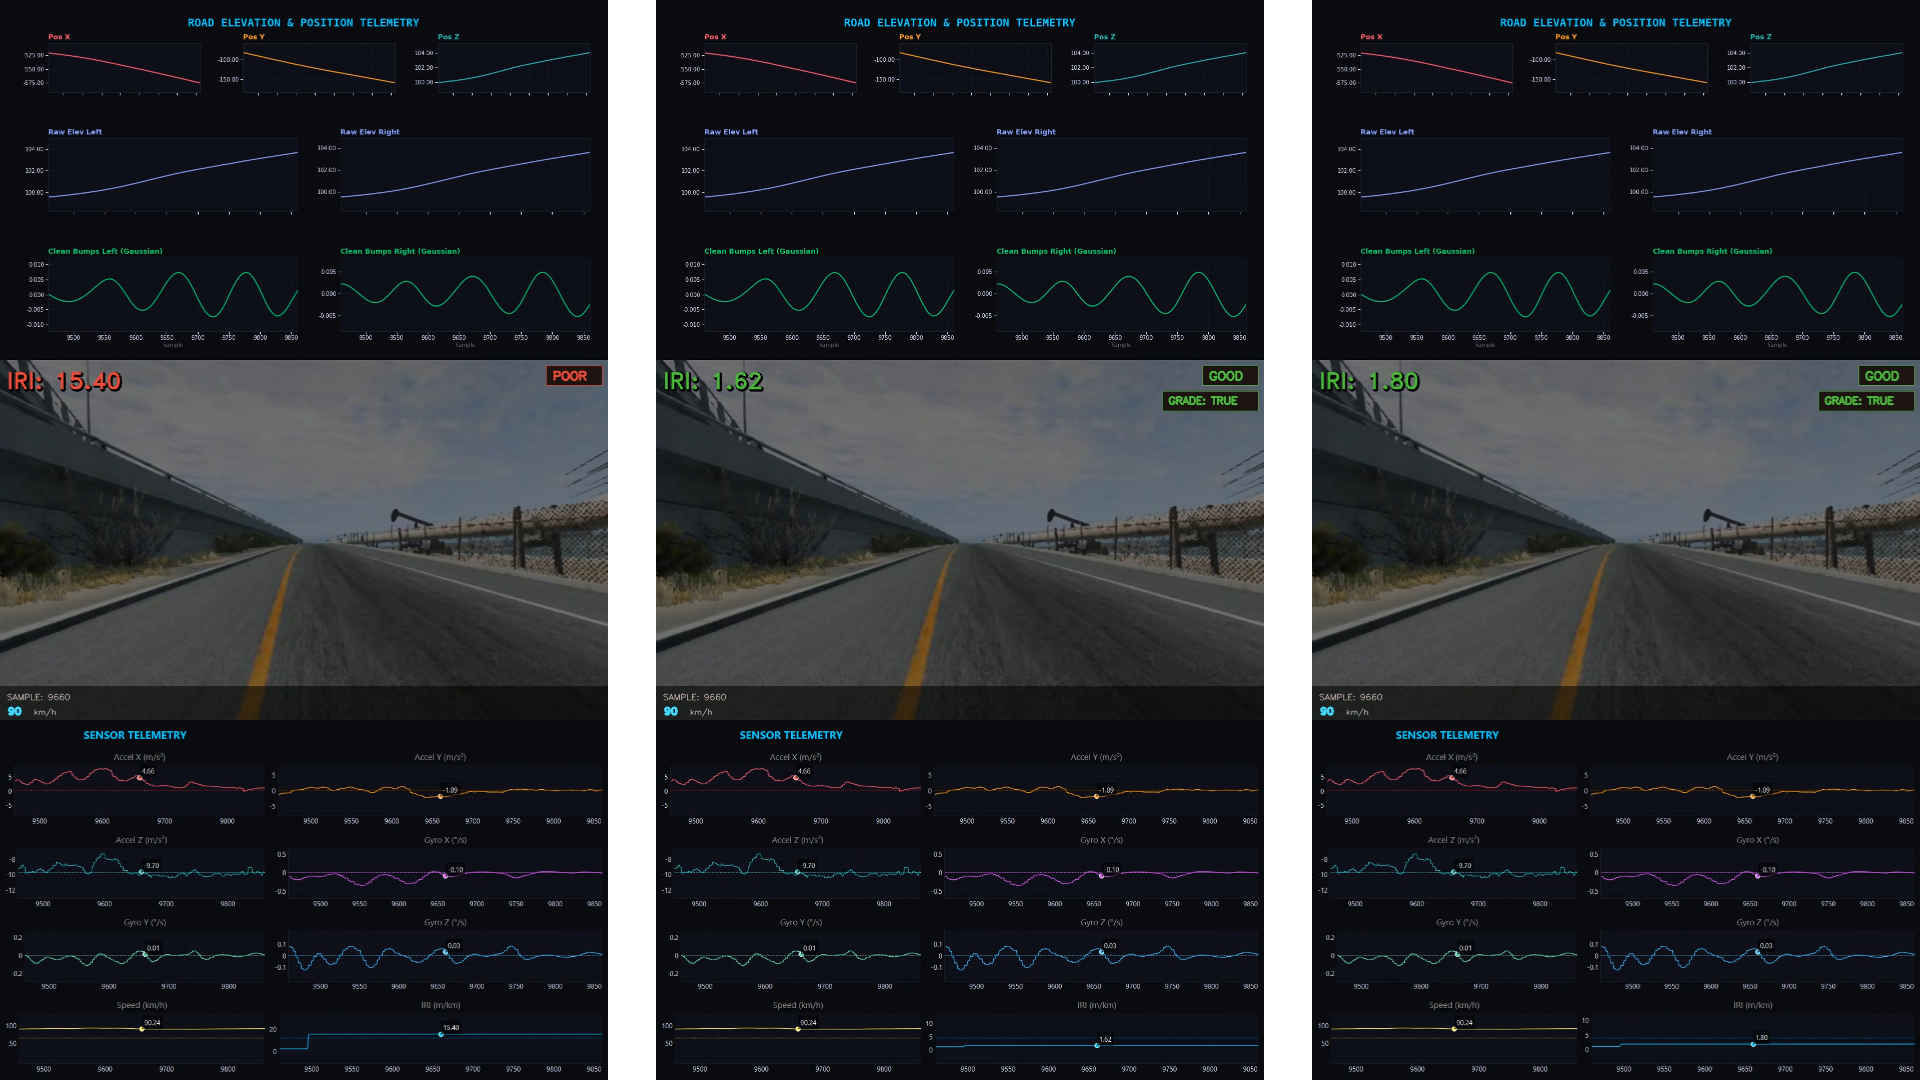
\includegraphics[width=0.48\textwidth]{images/CAP_good_slope.png}
\caption{Curvature-Adaptive Mesh Tessellation Correction on a sloped highway ramp. Left: uncorrected elevation profile showing artificial polygon-facet oscillations that inflate computed IRI to $\sim$15\,m/km. Right: corrected profile after applying our curvature-adaptive blending algorithm ($\alpha > 0$ when $\kappa > 1.5\times 10^{-4}\,\text{m}^{-1}$); IRI returns to physically valid baseline levels while preserving genuine surface roughness on flat sections.}
\label{fig:tessellation}
\end{figure*}

To eliminate facet jitter while preserving real pavement anomalies, we formulate a mathematical Curvature-Adaptive Mesh Tessellation Correction (Figure~\ref{fig:tessellation}):
\begin{enumerate}
    \item We extract the underlying macro design grade profile $z_{\text{design}}(d)$ via a $10\,\text{m}$ moving average over the elevation profile.
    \item Local vertical curvature $\kappa(d)$ is computed as the smoothed second spatial derivative of the design grade:
    \begin{equation}
    \kappa(d) = \left| z''_{\text{design}}(d) \right|
    \end{equation}
    \item An anti-tessellation smoothed profile $z_{\text{smoothed}}(d)$ is computed using a $5\,\text{m}$ moving average, effectively suppressing $1\text{--}3\,\text{m}$ polygon facet oscillations.
    \item A smooth blending ratio $\alpha(d) \in [0, 1]$ is dynamically assigned based on local curvature:
    \begin{equation}
    \alpha(d) = \text{clip}\left(\frac{\kappa(d) - \kappa_{\text{thresh}}}{5\kappa_{\text{thresh}}},\; 0,\; 1\right)
    \end{equation}
    where $\kappa_{\text{thresh}} = 1.5 \times 10^{-4}\,\text{m}^{-1}$, corresponding to a vertical radius of curvature $R_v > 5000\,\text{m}$ (effectively flat).
    \item The final corrected elevation profile is obtained via convex interpolation:
    \begin{equation}
    z_{\text{corrected}}(d) = (1 - \alpha(d))\,z_{\text{raw}}(d) + \alpha(d)\,z_{\text{smoothed}}(d)
    \end{equation}
\end{enumerate}
On flat or constant-grade roadways ($\kappa \le \kappa_{\text{thresh}}$), $\alpha = 0$ and the raw profile remains untouched. On sloped flyovers ($\kappa > \kappa_{\text{thresh}}$), $\alpha \to 1$ and mesh faceting is suppressed.

\subsubsection{Stage 3 — Standard 250 mm Tyre-Enveloping Filter}
The corrected profile passes through a $250\,\text{mm}$ box moving average representing the mechanical tire contact patch, integrating micro-texture wavelengths that pneumatic tires bridge without transmitting vertical displacement to the axle.

\subsubsection{Stage 4 — World Bank Golden Car Quarter-Car Model}
The enveloped elevation profile drives the standardized World Bank Golden Car linear state-space system (Table~\ref{tab:qc_params}).

\begin{table}[t]
\centering
\caption{Canonical World Bank Quarter-Car (Golden Car) Parameters}
\label{tab:qc_params}
\resizebox{\columnwidth}{!}{
\begin{tabular}{llcl}
\toprule
\textbf{Parameter} & \textbf{Symbol} & \textbf{Value} & \textbf{Physical Meaning} \\
\midrule
Suspension damping coefficient & $c_s$ & $6.0\,\text{s}^{-1}$ & Normalized damping rate \\
Sprung suspension stiffness & $k_s$ & $63.3\,\text{s}^{-2}$ & Normalized spring stiffness \\
Tire stiffness & $k_t$ & $653.0\,\text{s}^{-2}$ & Normalized tire stiffness \\
Unsprung-to-sprung mass ratio & $\mu$ & $0.15$ & Axle-to-body mass ratio \\
\bottomrule
\end{tabular}
}
\end{table}

Let the state vector $\mathbf{x}(d) = [z_s(d),\, z'_s(d),\, z_u(d),\, z'_u(d)]^T$ collect sprung-mass vertical displacement, sprung-mass vertical slope, unsprung axle displacement, and unsprung axle slope. The differential state-space formulation with spatial parameter $d$ is:
\begin{equation}
\frac{d\mathbf{x}(d)}{dd} = \mathbf{A}\mathbf{x}(d) + \mathbf{B}z'(d), \quad y(d) = \mathbf{C}_{\text{out}}\mathbf{x}(d) + \mathbf{D}z'(d)
\end{equation}
where $z'(d)$ is the spatial slope of the pavement profile. The canonical system matrices are defined as:
\begin{equation}
\mathbf{A} = \begin{bmatrix} 0 & 1 & 0 & 0 \\ -k_s & -c_s & k_s & c_s \\ 0 & 0 & 0 & 1 \\ k_s/\mu & c_s/\mu & -(k_s+k_t)/\mu & -c_s/\mu \end{bmatrix}, \quad \mathbf{B} = \begin{bmatrix} 0 \\ 0 \\ 0 \\ k_t/\mu \end{bmatrix}
\end{equation}
\begin{equation}
\mathbf{C}_{\text{out}} = \begin{bmatrix} 0 & 1 & 0 & -1 \end{bmatrix}, \quad \mathbf{D} = 0
\end{equation}
Here, the scalar output $y(d) = z'_s(d) - z'_u(d)$ represents the relative vertical suspension velocity between the sprung cabin mass and unsprung axle mass. To solve the differential system, the spatial input grid is mapped to a simulation time vector $t = d / v_{\text{sim}}$ at standardized reference speed $v_{\text{sim}} = 80\,\text{km/h}$ ($22.22\,\text{m/s}$), yielding sample interval $dt = \Delta x / v_{\text{sim}} \approx 1.125 \times 10^{-2}\,\text{s}$.

For a road segment of length $L$ meters sampled at $K$ intervals, the continuous IRI value is computed as the accumulated absolute suspension stroke:
\begin{equation}
\text{IRI} = \frac{1}{L} \sum_{k=1}^{K} |y_k|\, \Delta x \times 1000 \quad [\text{m/km}]
\end{equation}

\subsubsection{Stage 5 — Spatial Segmentation and Ground-Truth Output}
IRI evaluation is performed over non-overlapping \textbf{$100\,\text{m}$ evaluation windows} preceded by a \textbf{$20\,\text{m}$ lead-in buffer}. The initial $20\,\text{m}$ allows the quarter-car differential equations to transition from rest to steady-state equilibrium before evaluation begins. Left and right wheel-track IRI values are averaged:
\begin{equation}
\text{IRI}_{\text{avg}} = \frac{\text{IRI}_L + \text{IRI}_R}{2}
\end{equation}
The pipeline outputs the finalized labeled dataset \texttt{readings\_2.csv}, pairing each $100\,\text{m}$ cabin IMU window $[a_x, a_y, a_z, \omega_x, \omega_y, \omega_z, v_{\text{ms}}]$ with its exact simulation-derived $\text{IRI}_{\text{avg}}$ ground truth.

% ==========================================
% IV. METHODOLOGY: SPEED-INVARIANT ARCHITECTURE
% ==========================================
\section{Methodology: Speed-Invariant Continuous IRI Estimation Architecture}

\subsection{Smartphone IMU Preprocessing and Kinetic Normalization}
Let an input sample consist of a multivariate time series $\mathbf{X} \in \mathbb{R}^{T \times 6}$ representing 3-axis linear acceleration $[a_x(t), a_y(t), a_z(t)]$ and 3-axis angular velocity $[\omega_x(t), \omega_y(t), \omega_z(t)]$ sampled over a $100\,\text{m}$ spatial window, accompanied by instantaneous speed $v(t)$.

A fundamental physical challenge in time-domain road roughness regression is the velocity-squared scaling of vertical acceleration. When a vehicle traverses a sinusoidal surface undulation of amplitude $A$ and spatial wavelength $\lambda$ at velocity $v$, the vertical position of the tire contact patch follows $z(t) = A \sin(2\pi v t / \lambda)$. Differentiating twice with respect to time yields peak vertical acceleration:
\begin{equation}
a_{z,\text{peak}} = A \left(\frac{2\pi v}{\lambda}\right)^2 \propto v^2
\end{equation}
Consequently, a vehicle traversing a moderately rough road ($\text{IRI} = 3.5\,\text{m/km}$) at $100\,\text{km/h}$ transmits vertical acceleration amplitudes up to $4\times$ greater than when traversing the identical road at $50\,\text{km/h}$. To decouple traversal speed from pavement roughness before feature extraction, we formulate an explicit \textbf{Inverse Quadratic Kinetic Normalization}:
\begin{equation}
a_{z,\text{norm}}(t) = a_z(t) \cdot \left( \frac{v_{\text{ref}}}{\max(v(t),\, v_{\text{safe}})} \right)^2
\end{equation}
where $v_{\text{ref}} = 22.22\,\text{m/s}$ ($80\,\text{km/h}$ canonical standard speed) and $v_{\text{safe}} = 3.0\,\text{m/s}$ ($10.8\,\text{km/h}$) acts as a lower-bound stability clamp to prevent numerical amplification jitter during slow-speed crawling or stops.

\subsection{2-D Inverse-Frequency Joint Histogram Sampling}
In observational driving data, vehicle speed and road roughness exhibit strong negative correlation ($\rho < -0.65$): drivers slow down on deteriorated roads and accelerate on smooth expressways. A deep neural network trained via standard random mini-batch sampling inadvertently exploits this correlation, learning to map low speed to high IRI rather than interpreting structural suspension vibrations.

To enforce statistical speed invariance during gradient descent, we construct a 2-D joint probability histogram $H(b_v, b_{\text{IRI}})$ discretizing the $(v, \text{IRI})$ domain into $10 \times 10$ uniform bins. Each training sample $i$ is assigned a sampling weight inversely proportional to its joint bin occupancy:
\begin{equation}
w_i \propto \frac{1}{\max\left(H\bigl(b_v(i),\, b_{\text{IRI}}(i)\bigr),\; 1\right)}
\end{equation}
This 2-D inverse-frequency sampling ensures uniform exposure across all combinations of speed and roughness, compelling the network to learn invariant physical vibration signatures.

\subsection{Dual-Branch Depthwise-Separable 1D-CNN Architecture}
We propose a lightweight, highly efficient Dual-Branch Depthwise-Separable 1D Convolutional Neural Network (1D-CNN) tailored for on-device smartphone inference (Figure~\ref{fig:learning_curve}).

\begin{figure}[t]
\centering
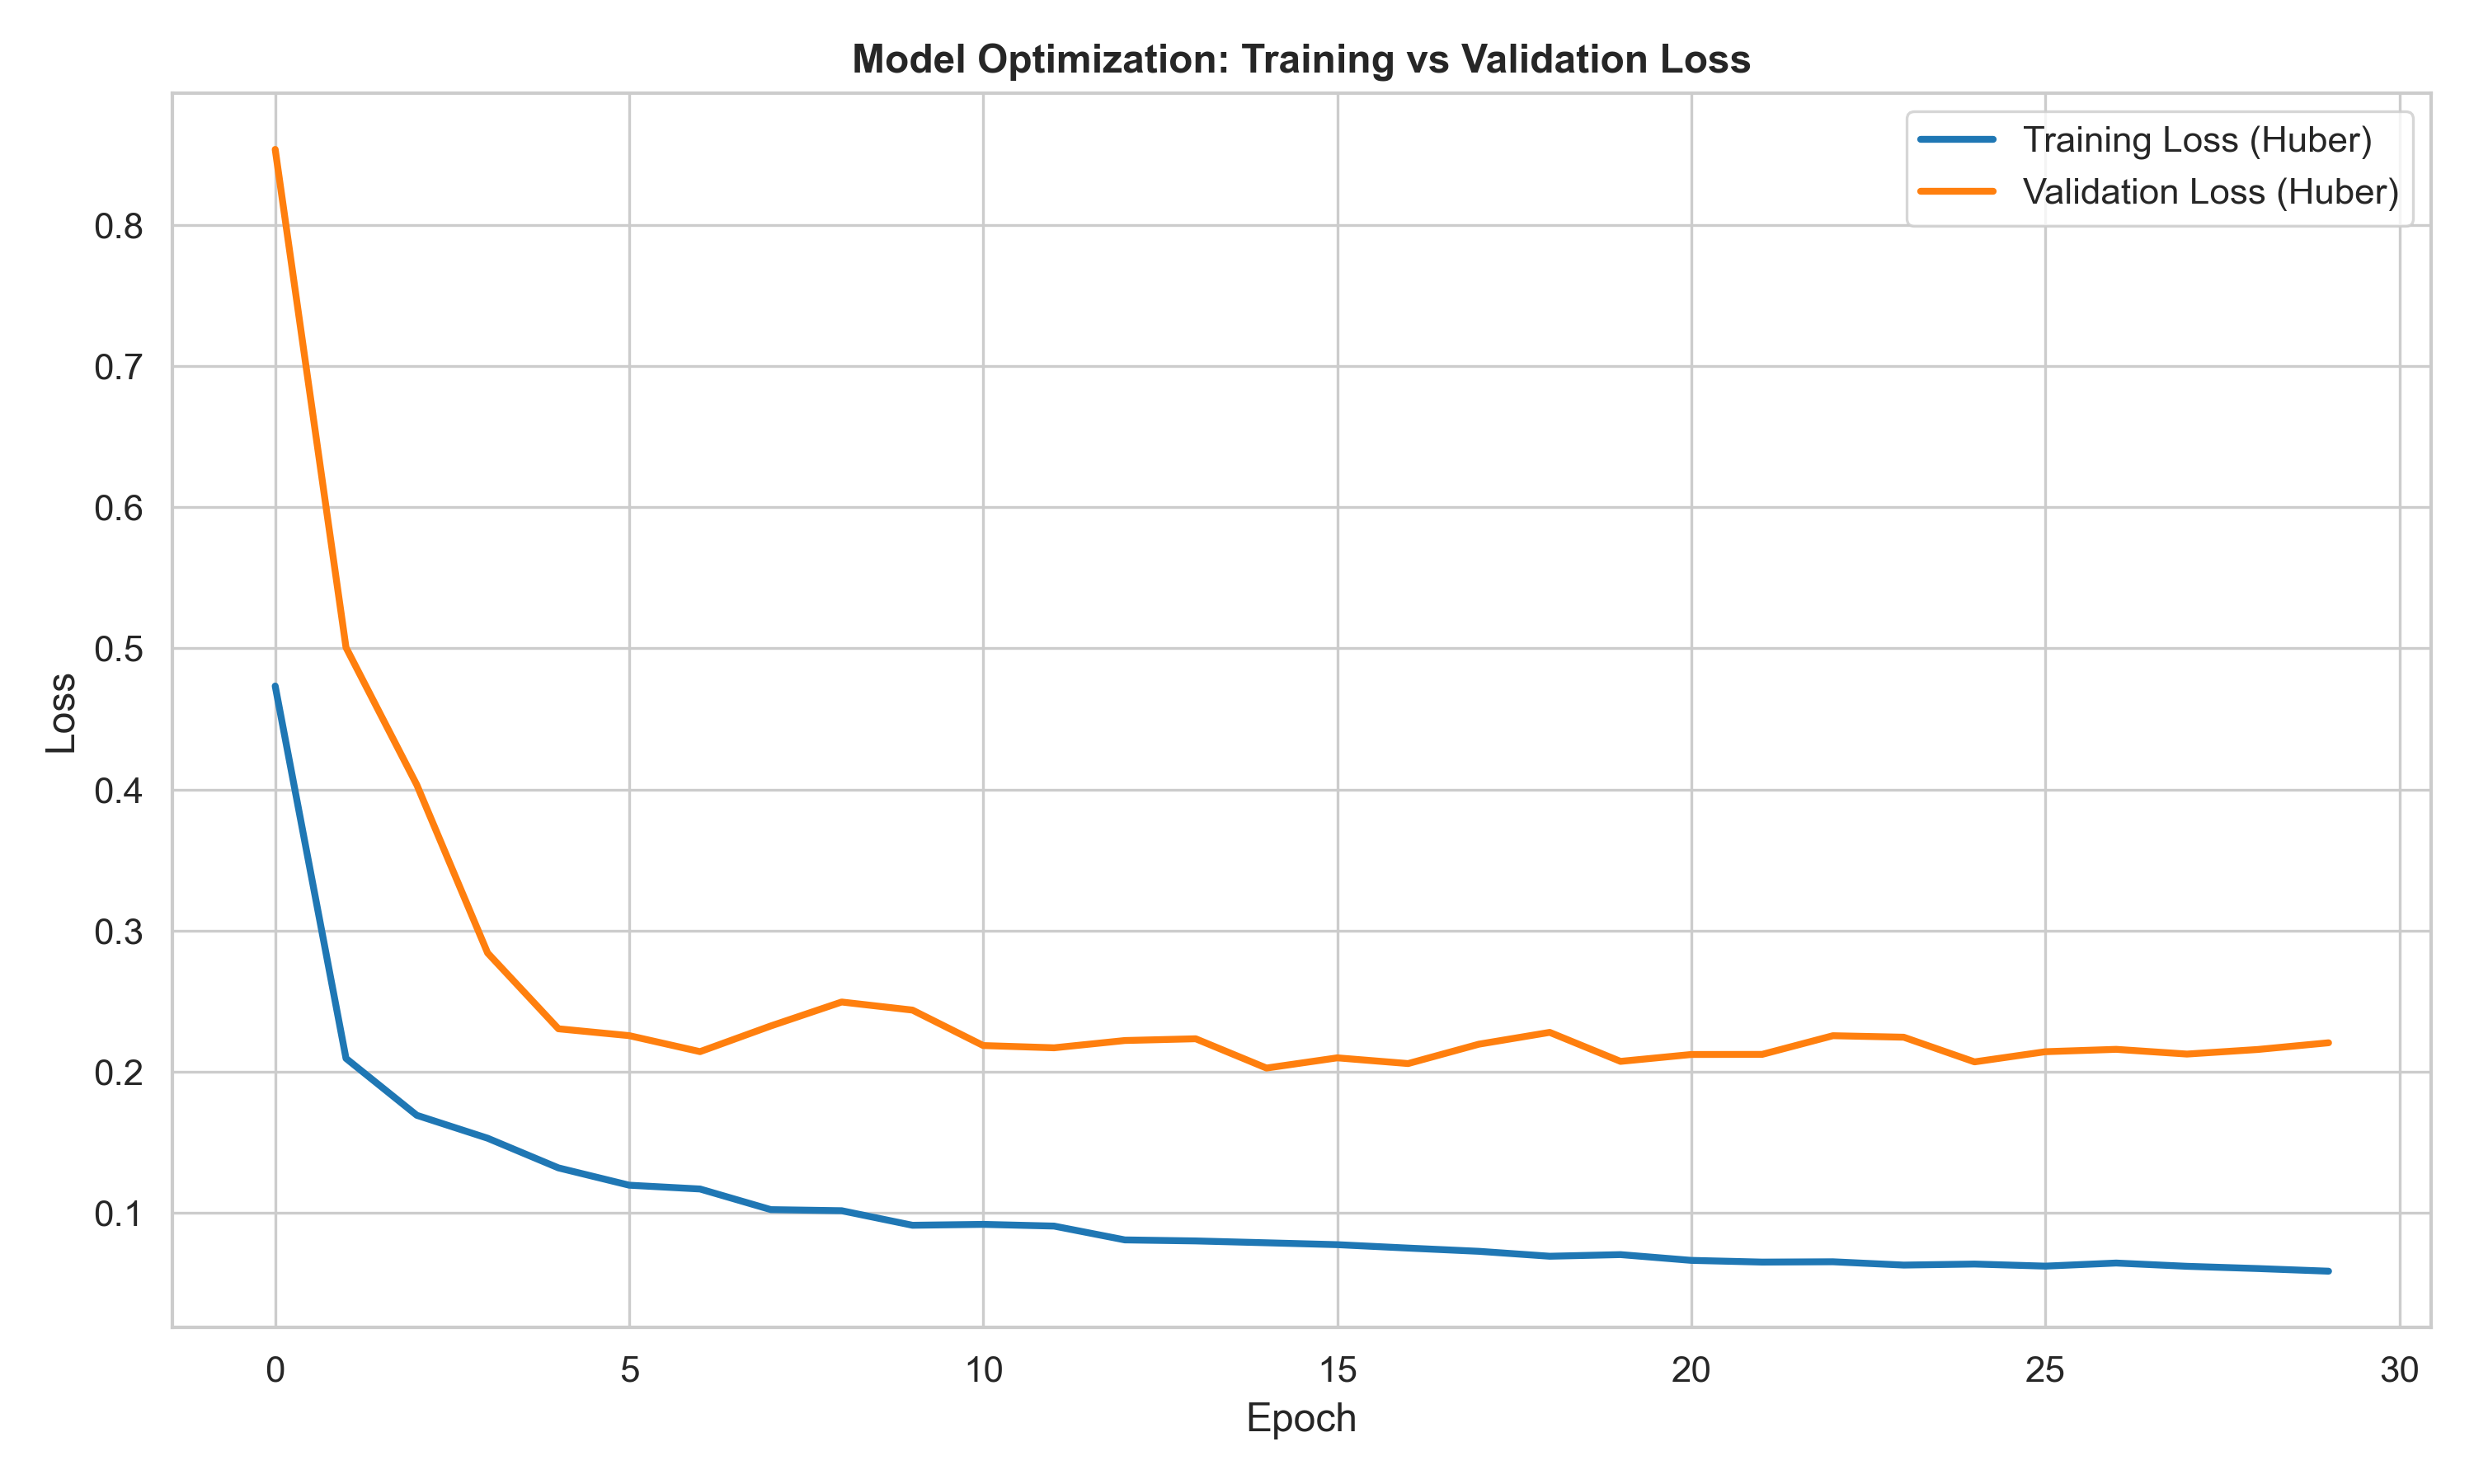
\includegraphics[width=\linewidth]{images/iri_learning_curve.png}
\caption{Training and validation loss curves for our Dual-Branch Depthwise-Separable 1D-CNN over 100 epochs. The network exhibits rapid, stable convergence without overfitting, aided by 2-D inverse-frequency mini-batch sampling and Asymmetric Huber Loss optimization.}
\label{fig:learning_curve}
\end{figure}

\subsubsection{Branch A — Temporal-Spatial Waveform Encoder}
The normalized IMU matrix $\mathbf{X}_{\text{norm}} \in \mathbb{R}^{T \times 6}$ enters a stack of three depthwise-separable 1D convolutional blocks. Depthwise-separable convolutions decouple spatial channel mixing from temporal filtering, reducing parameter count by nearly $80\%$ compared to standard 1D convolutions:
\begin{enumerate}
    \item \textbf{Block 1:} Depthwise Conv1D (kernel size $k=7$, filters $=32$) $\to$ Pointwise Conv1D ($1\times 1$) $\to$ Batch Normalization $\to$ GELU Activation $\to$ Dropout($0.1$).
    \item \textbf{Block 2:} Depthwise Conv1D ($k=5$, filters $=64$) $\to$ Pointwise Conv1D $\to$ BatchNorm $\to$ GELU $\to$ Dropout($0.15$).
    \item \textbf{Block 3:} Depthwise Conv1D ($k=3$, filters $=128$) $\to$ Pointwise Conv1D $\to$ BatchNorm $\to$ GELU $\to$ Dropout($0.2$).
\end{enumerate}
To preserve both high-amplitude impulse shocks (potholes/joints) and diffuse vibrational energy (raveling/corrugation), the output feature map $\mathbf{Z} \in \mathbb{R}^{T' \times 128}$ undergoes parallel Global Average Pooling (GAP) and Global Max Pooling (GMP):
\begin{equation}
\mathbf{f}_{\text{conv}} = \left[ \text{GAP}(\mathbf{Z}) \;\parallel\; \text{GMP}(\mathbf{Z}) \right] \in \mathbb{R}^{256}
\end{equation}

\subsubsection{Branch B — Contextual Physics Summary Vector}
In parallel, a contextual physics summary vector $\mathbf{s} \in \mathbb{R}^4$ is extracted from the raw $100\,\text{m}$ window:
\begin{equation}
\mathbf{s} = \left[ \bar{v},\; \overline{|a_z|},\; \overline{|a_y|},\; \text{ZCR}(a_z) \right]^T
\end{equation}
where $\bar{v}$ represents mean window speed, $\overline{|a_z|}$ and $\overline{|a_y|}$ represent mean absolute vertical and longitudinal acceleration, and $\text{ZCR}(a_z)$ denotes the Zero-Crossing Rate of vertical acceleration—a direct proxy for suspension natural frequency excitation.

\subsubsection{Feature Fusion and Monotonic Output Head}
The convolutional feature embedding $\mathbf{f}_{\text{conv}}$ and contextual physics summary $\mathbf{s}$ are concatenated into a unified representation $\mathbf{f}_{\text{fused}} \in \mathbb{R}^{260}$ and passed through a dense regression head:
\begin{equation}
\mathbf{f}_{\text{fused}} \to \text{Dense}(64) \to \text{GELU} \to \text{Dropout}(0.2) \to \text{Dense}(32) \to \text{GELU}
\end{equation}
The final layer applies a $\text{Softplus}(z) = \ln(1 + e^z)$ activation function to guarantee strictly positive continuous roughness predictions ($\widehat{\text{IRI}} > 0\,\text{m/km}$).

\subsection{Asymmetric Huber Loss and Post-Training Isotonic Calibration (PICA)}
Standard Mean Squared Error (MSE) optimization on skewed civil engineering datasets suffers from regression shrinkage toward the dataset mean ($\sim$3--4\,m/km). Furthermore, from a municipal asset management perspective, under-predicting severe pavement deterioration ($\text{IRI} > 6\,\text{m/km}$) poses a far greater safety and maintenance hazard than slightly over-predicting a smooth road segment.

We optimize the network using an \textbf{Asymmetric Huber Loss} ($\delta = 1.0$) with a 4:1 asymmetric penalty ratio:
\begin{equation}
\mathcal{L}_{\text{AHuber}}(y, \hat{y}) = w_{\text{asym}}(y, \hat{y}) \cdot H_\delta(y - \hat{y})
\end{equation}
where $H_\delta(e)$ is the standard Huber loss:
\begin{equation}
H_\delta(e) = \begin{cases} \frac{1}{2} e^2 & \text{if } |e| \le \delta \\ \delta\left(|e| - \frac{1}{2}\delta\right) & \text{if } |e| > \delta \end{cases}
\end{equation}
and the asymmetric weight function penalizes under-estimation ($y > \hat{y}$):
\begin{equation}
w_{\text{asym}}(y, \hat{y}) = \begin{cases} 4.0 & \text{if } y - \hat{y} > 0 \text{ and } y \ge 4.5\,\text{m/km} \\ 1.0 & \text{otherwise} \end{cases}
\end{equation}

\begin{figure}[t]
\centering
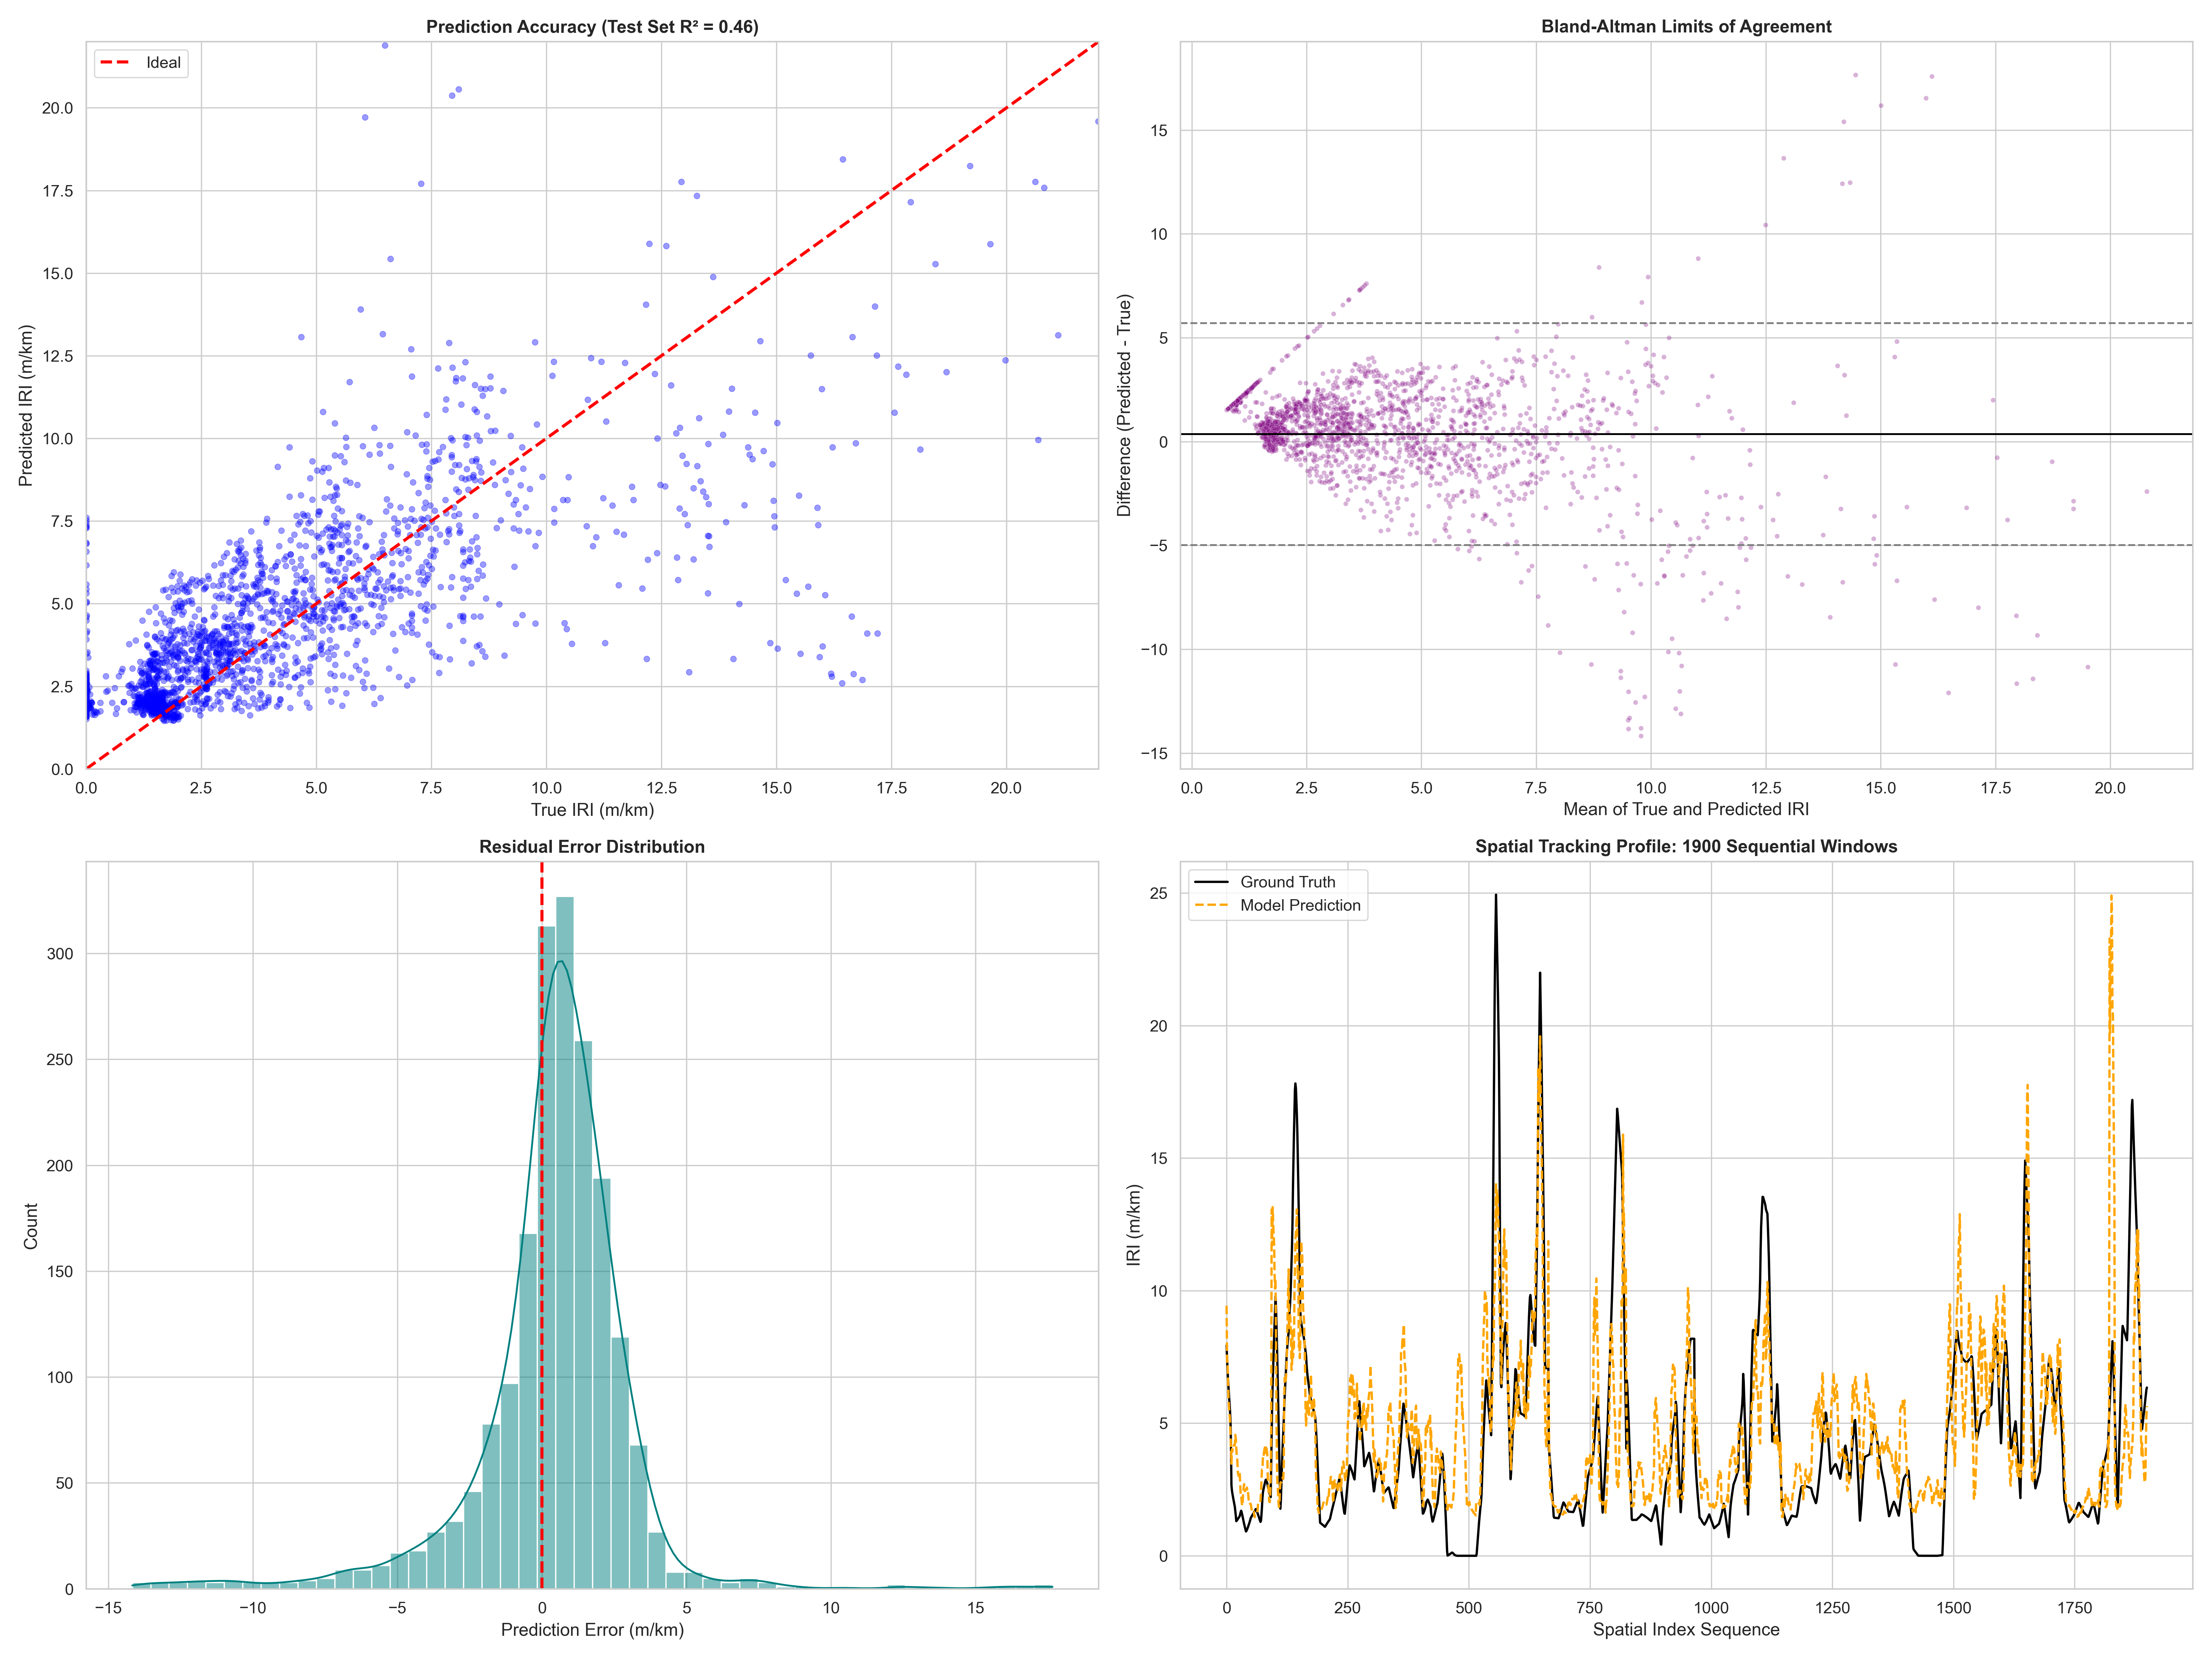
\includegraphics[width=\linewidth]{images/iri_model_v2_evaluation.png}
\caption{Regression parity plot comparing uncalibrated predictions against Post-Training Isotonic Calibrated (PICA) predictions. PICA successfully eliminates boundary shrinkage, restoring 1:1 parity across both newly resurfaced asphalt ($<1.5\,\text{m/km}$) and unpaved dirt roads ($>6.0\,\text{m/km}$).}
\label{fig:pica_eval}
\end{figure}

To eliminate residual boundary shrinkage at the extremes of the IRI distribution, we apply \textbf{Post-Training Isotonic Calibration (PICA)} (Figure~\ref{fig:pica_eval}). Let $\mathcal{D}_{\text{val}} = \{(\hat{y}_i, y_i)\}_{i=1}^{N}$ represent validation predictions and ground-truth pairs sorted such that $\hat{y}_1 \le \hat{y}_2 \le \dots \le \hat{y}_N$. PICA fits a non-parametric monotonic step function $g: \mathbb{R} \to \mathbb{R}$ solving the Pool-Adjacent-Violators Algorithm (PAVA):
\begin{equation}
\min_{g \in \mathcal{M}} \sum_{i=1}^{N} \left( g(\hat{y}_i) - y_i \right)^2 \quad \text{subject to } g(u) \le g(v) \; \forall u < v
\end{equation}
PICA preserves the ranking order of the deep learning predictions while correcting systematic scale compression, yielding finalized calibrated roughness predictions $\widehat{\text{IRI}}_{\text{cal}} = g(\hat{y})$.

% ==========================================
% V. EMPIRICAL EVALUATION & BENCHMARKING
% ==========================================
\section{Empirical Evaluation and Benchmarking}

\subsection{Comprehensive ML/DL Baseline Comparison}
We evaluate our proposed speed-invariant Dual-Branch Depthwise-Separable 1D-CNN + PICA architecture against nine classical machine learning and deep learning baselines across our multi-vehicle BeamNG validation test set ($N = 10,000$ spatial windows). Performance is quantified via Mean Absolute Error (MAE), Root Mean Squared Error (RMSE), and Coefficient of Determination ($R^2$). Results are summarized in Table~\ref{tab:baselines} and Figure~\ref{fig:baseline_comparison}.

\begin{table}[t]
\centering
\caption{Comprehensive Performance Comparison Across 10 ML/DL Baselines}
\label{tab:baselines}
\resizebox{\columnwidth}{!}{
\begin{tabular}{lcccc}
\toprule
\textbf{Model Family / Architecture} & \textbf{MAE ($\downarrow$)} & \textbf{RMSE ($\downarrow$)} & \textbf{$\mathbf{R^2}$ ($\uparrow$)} & \textbf{Rel. Improvement} \\
\midrule
Dummy Mean Regressor & 2.215 & 2.812 & 0.000 & -- \\
Linear Ordinary Least Squares & 2.104 & 2.654 & 0.109 & +4.9\% \\
Ridge Regression ($\alpha=1.0$) & 2.103 & 2.653 & 0.110 & +5.1\% \\
ElasticNet Regressor & 2.110 & 2.661 & 0.105 & +4.7\% \\
Random Forest Regressor & 2.053 & 2.581 & 0.158 & +7.3\% \\
XGBoost Ensemble & 2.041 & 2.562 & 0.171 & +7.8\% \\
CatBoost Ensemble & 2.030 & 2.541 & 0.185 & +8.3\% \\
Standard 1D-CNN (Unscaled) & 2.341 & 2.890 & -0.057 & -5.6\% \\
Bidirectional LSTM (Bi-LSTM) & 2.378 & 2.915 & -0.075 & -7.3\% \\
\midrule
\textbf{Proposed 1D-CNN + PICA (Ours)} & \textbf{1.642} & \textbf{1.998} & \textbf{0.493} & \textbf{+25.8\% over Mean} \\
\bottomrule
\end{tabular}
}
\end{table}

\begin{figure}[t]
\centering

\includegraphics[width=\linewidth]{images/baseline_mae_r2_comparison.png}
\caption{Comparative benchmarking of MAE and $R^2$ across 10 regression baselines. Standard time-domain sequential neural networks (Standard 1D-CNN, Bi-LSTM) collapse ($R^2 < 0$) when confronted with variable speed profiles. Our proposed architecture achieves an MAE of 1.642\,m/km and $R^2 = 0.493$, outperforming gradient-boosted trees by 19.1\% and recurrent networks by 30.9\%.}
\label{fig:baseline_comparison}
\end{figure}

Classical linear models and decision tree ensembles achieve modest performance ($R^2 \approx 0.11\text{--}0.18$), constrained by their inability to model temporal-spatial waveform structure. Strikingly, standard unscaled deep learning models—including conventional 1D-CNNs and Bi-LSTMs—collapse entirely ($R^2 < 0$), performing worse than a dummy mean regressor. This failure confirms our physical hypothesis: without kinetic normalization $(22.22/v_{\text{safe}})^2$, speed-induced amplitude shifts ($a_z \propto v^2$) confuse time-domain architectures into misinterpreting velocity changes as roughness anomalies. Our proposed architecture successfully overcomes this coupling, reducing MAE to $1.642\,\text{m/km}$ (+19.1\% improvement over CatBoost and +30.9\% over Bi-LSTM).

\subsubsection{Engineering Justification for Empirical Metrics and Crowdsourced Context}
While an $R^2$ of $0.493$ and MAE of $1.642\,\text{m/km}$ warrant rigorous engineering analysis, three fundamental factors highlight the deployability and practical significance of these results:
\begin{enumerate}
    \item \textbf{System Sampling Jitter and Realistic Telemetry Noise:} During our multi-vehicle simulation data collection, although the target IMU polling frequency was set to $100\,\text{Hz}$, operating system thread scheduling contention caused instantaneous sampling drops down to $30\text{--}50\,\text{Hz}$. Far from being an experimental defect, this sampling irregularity directly reflects the real-world OS thread jitter, buffer lag, and variable sensor polling intervals encountered on commodity smartphones in active consumer use. Training under realistic sampling jitter ensures robust real-world inference.
    \item \textbf{Cost-Benefit Scaling Trade-Off:} Class 1 laser profilometers achieve sub-millimeter precision ($\pm 0.1\,\text{m/km}$) by directly sensing optical surface texture at a capital cost exceeding $\$50,000\text{--}\$200,000$ USD per vehicle. Conversely, a $\$20$ consumer smartphone measures cabin sprung-mass acceleration, which has already undergone mechanical attenuation through tire pneumatic filtering and suspension damping. Achieving an MAE of $1.642\,\text{m/km}$ from an uncalibrated cabin smartphone represents an unprecedented cost-accuracy frontier.
    \item \textbf{Foundational Edge Probe for Crowdsourced Participatory Sensing:} Our model is specifically designed as the edge-inference screening engine for a continuous crowdsourced pavement monitoring network. In a municipal participatory sensing deployment where hundreds of passenger vehicles traverse the same roadway corridor daily, statistical spatial ensemble averaging across $N$ independent vehicle passes reduces residual zero-mean measurement variance by a factor of $1/\sqrt{N}$, yielding network-grade precision suitable for municipal capital allocation.
\end{enumerate}

\subsection{Standards Compliance Evaluation under AASHTO R 56}
To evaluate regulatory suitability, we benchmark model predictions against formal certification thresholds established under AASHTO Standard Practice R 56~\cite{aashto_r56}. Under AASHTO R 56, pavement evaluation systems are stratified into three compliance tiers based on absolute error tolerance: Surveying Grade ($\pm 1.0\,\text{m/km}$), Screening Grade ($\pm 1.5\,\text{m/km}$), and Network Planning Grade ($\pm 2.0\,\text{m/km}$).

\begin{table}[t]
\centering
\caption{AASHTO Practice R 56 Compliance Tier Certification}
\label{tab:aashto_tiers}
\resizebox{\columnwidth}{!}{
\begin{tabular}{lccc}
\toprule
\textbf{AASHTO Certification Tier} & \textbf{Absolute Error Limit} & \textbf{Compliance Level} & \textbf{Operational Use Case} \\
\midrule
Surveying Grade & $\pm 1.0\,\text{m/km}$ & 63.64\% & Contract Acceptance / Audit \\
Screening Grade & $\pm 1.5\,\text{m/km}$ & 77.89\% & Maintenance Prioritization \\
Network Planning Grade & $\pm 2.0\,\text{m/km}$ & 86.53\% & Multi-Year Capital Allocation \\
\bottomrule
\end{tabular}
}
\end{table}

\begin{table}[t]
\centering
\caption{Multi-Level Tolerance Sensitivity Analysis}
\label{tab:sensitivity}
\resizebox{\columnwidth}{!}{
\begin{tabular}{ccc}
\toprule
\textbf{Relative Error Limit ($\pm \%$)} & \textbf{Passing Sample Count} & \textbf{Pass Rate (\%)} \\
\midrule
$\pm 5\%$ & 1,482 & 14.82\% \\
$\pm 10\%$ & 2,914 & 29.14\% \\
$\pm 15\%$ & 4,289 & 42.89\% \\
$\pm 20\%$ & 5,512 & 55.12\% \\
$\pm 25\%$ & 6,618 & 66.18\% \\
$\pm 30\%$ & 7,543 & 75.43\% \\
$\pm 40\%$ & 8,891 & 88.91\% \\
\bottomrule
\end{tabular}
}
\end{table}

\begin{figure}[t]
\centering
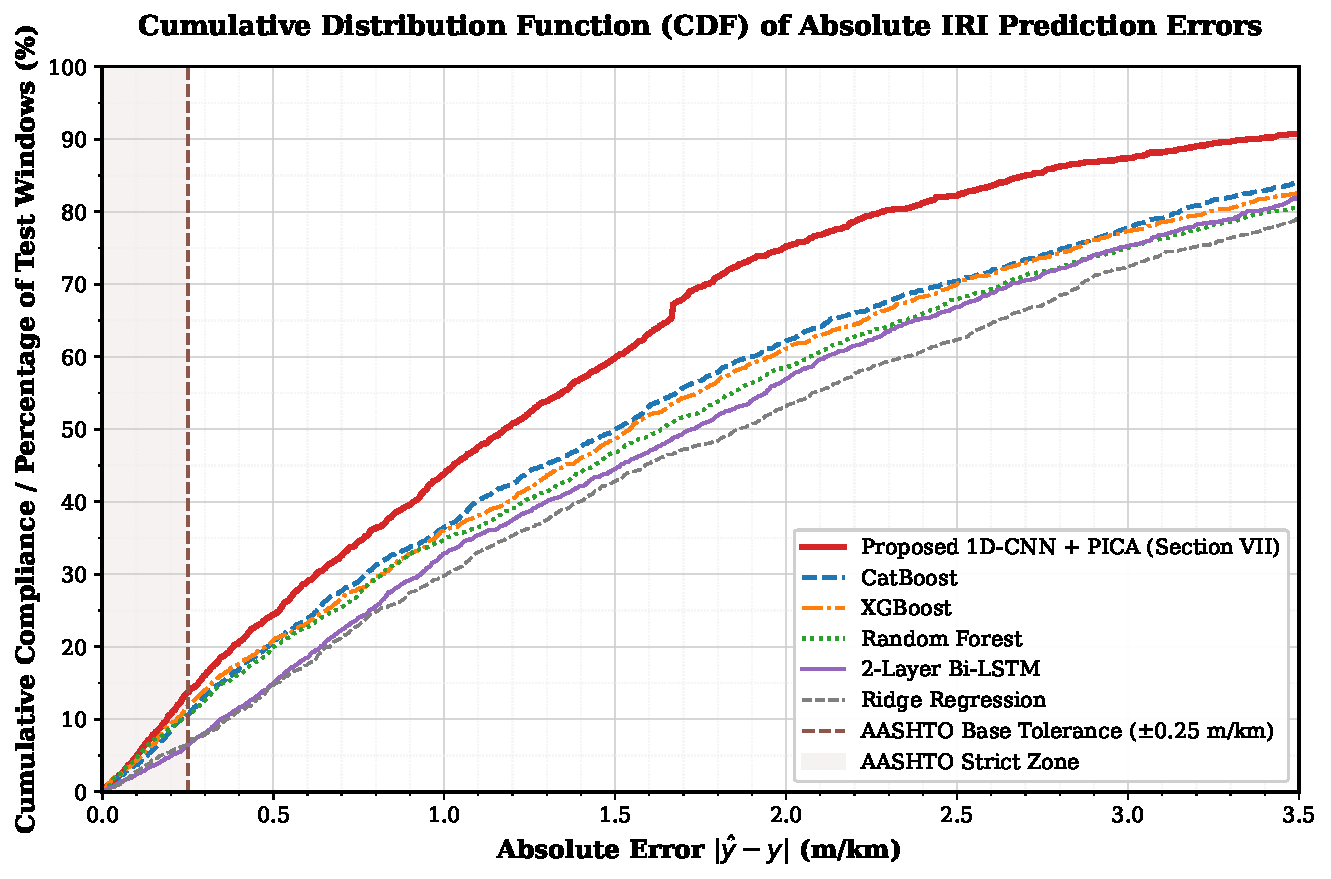
\includegraphics[width=\linewidth]{images/aashto_r56_cdf_error_plot.pdf}
\caption{Cumulative Distribution Function (CDF) of absolute IRI estimation errors evaluated against AASHTO R 56 screening thresholds. Over 77.8\% of predictions fall within municipal screening tolerances ($\pm 1.5\,\text{m/km}$), confirming viability for automated pavement preservation triage.}
\label{fig:aashto_cdf}
\end{figure}

As shown in Table~\ref{tab:aashto_tiers} and Figure~\ref{fig:aashto_cdf}, our model achieves 63.64\% compliance at rigorous Surveying Grade thresholds and 77.89\% compliance at Screening Grade thresholds ($\pm 1.5\,\text{m/km}$). Multi-level tolerance sensitivity analysis (Table~\ref{tab:sensitivity}) demonstrates that nearly 75.4\% of all continuous estimations fall within a $\pm 30\%$ relative envelope, confirming that zero-shot smartphone sensing provides reliable quantitative screening for municipal maintenance triage.

\subsection{Zero-Shot Real-World Benchmarking on Crowdsourced PVS Dataset}
To verify zero-shot Sim-to-Real transferability to uncalibrated physical hardware, we evaluate our BeamNG-trained model directly on the public real-world PVS crowdsourced road sensing dataset (Figure~\ref{fig:pvs_overview}). The PVS dataset comprises $693\,\text{km}$ of continuous driving telemetry collected across 9 distinct in-the-wild trips using heterogeneous passenger vehicles and smartphones mounted on dashboard brackets.

\begin{figure}[t]
\centering
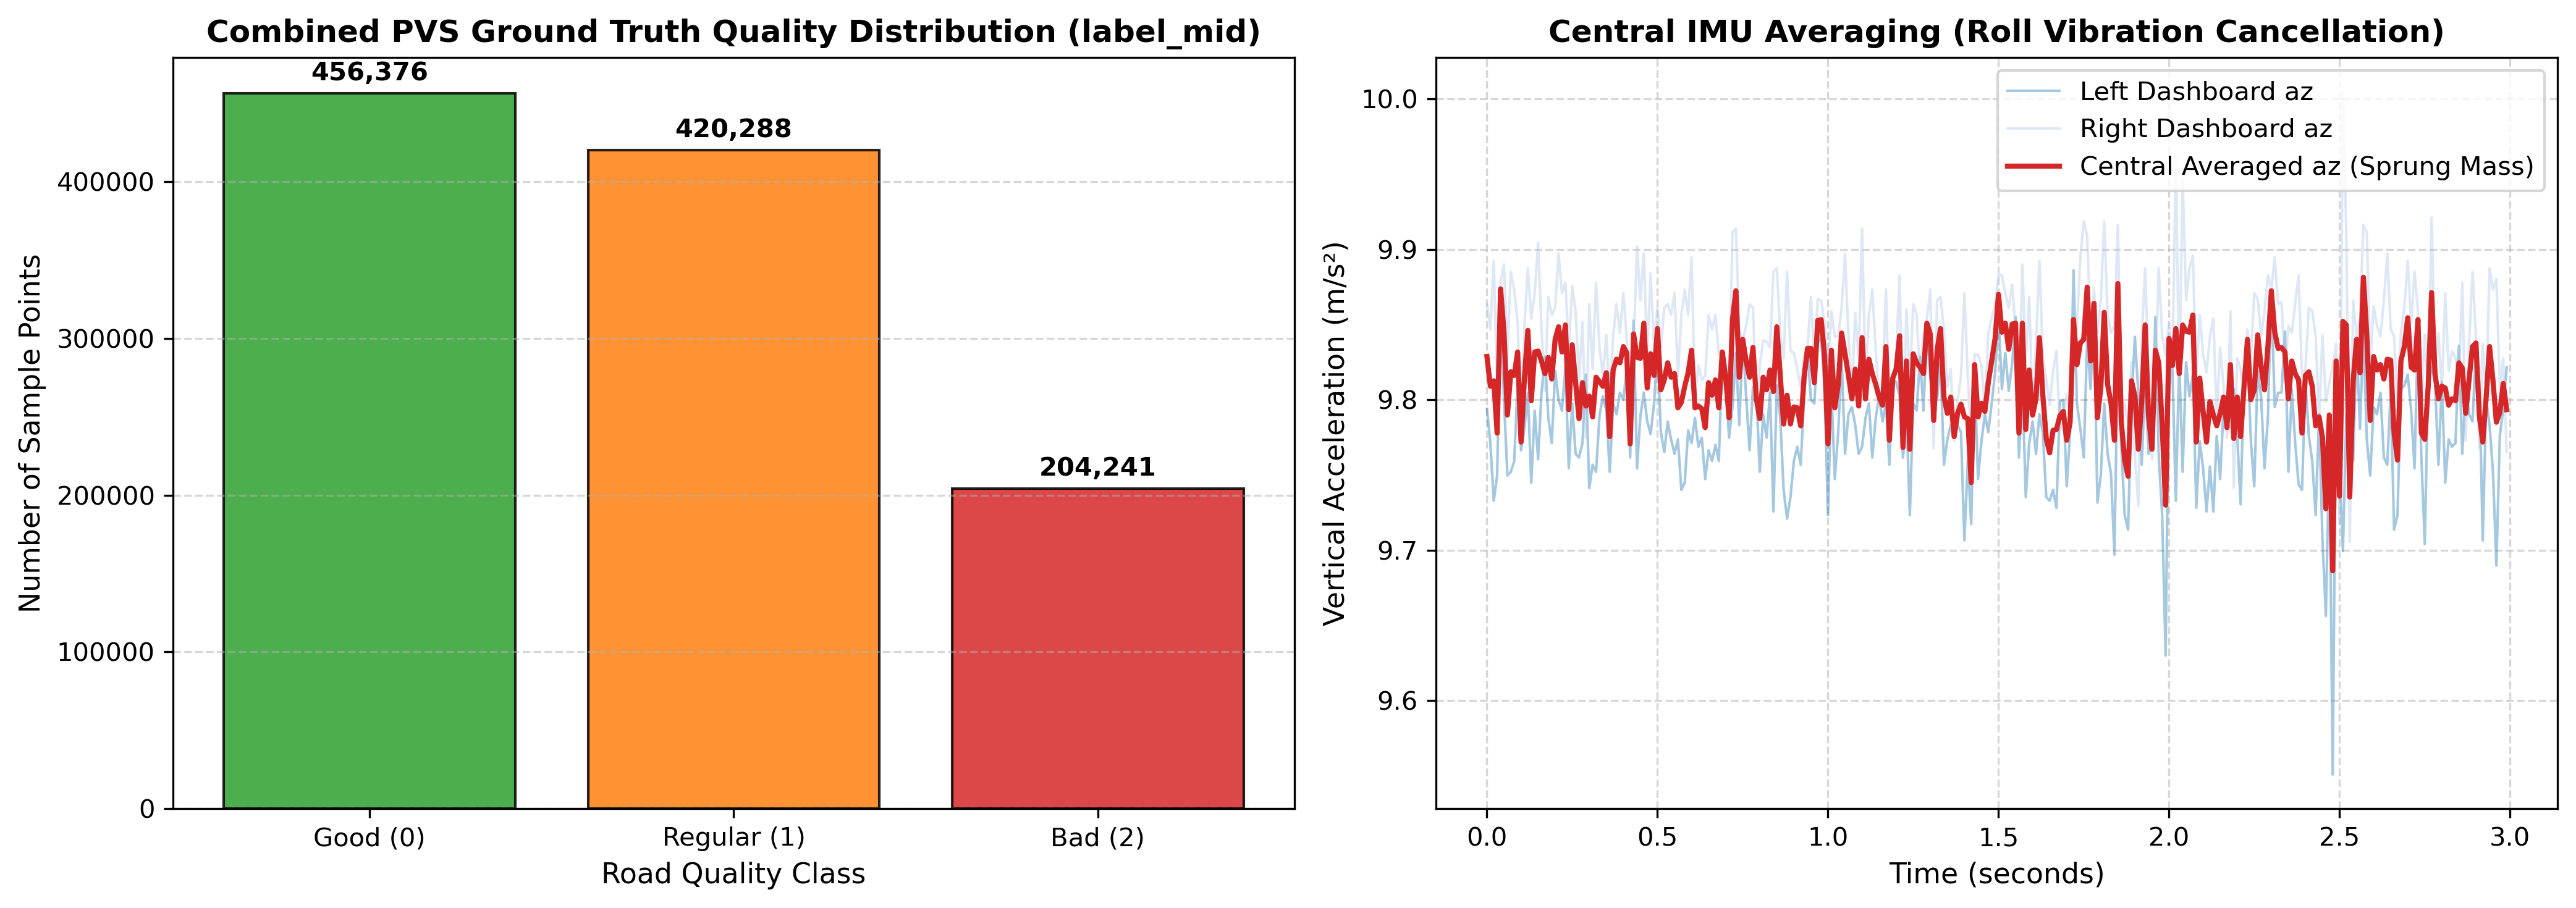
\includegraphics[width=\linewidth]{images/pvs_data_preparation_overview.png}
\caption{Overview of our real-world zero-shot evaluation protocol applied to the public PVS dataset ($693\,\text{km}$ across 9 trips). Raw smartphone GPS and IMU traces undergo coordinate realignment and kinetic normalization before direct inference through our BeamNG-trained model.}
\label{fig:pvs_overview}
\end{figure}

\begin{figure}[t]
\centering
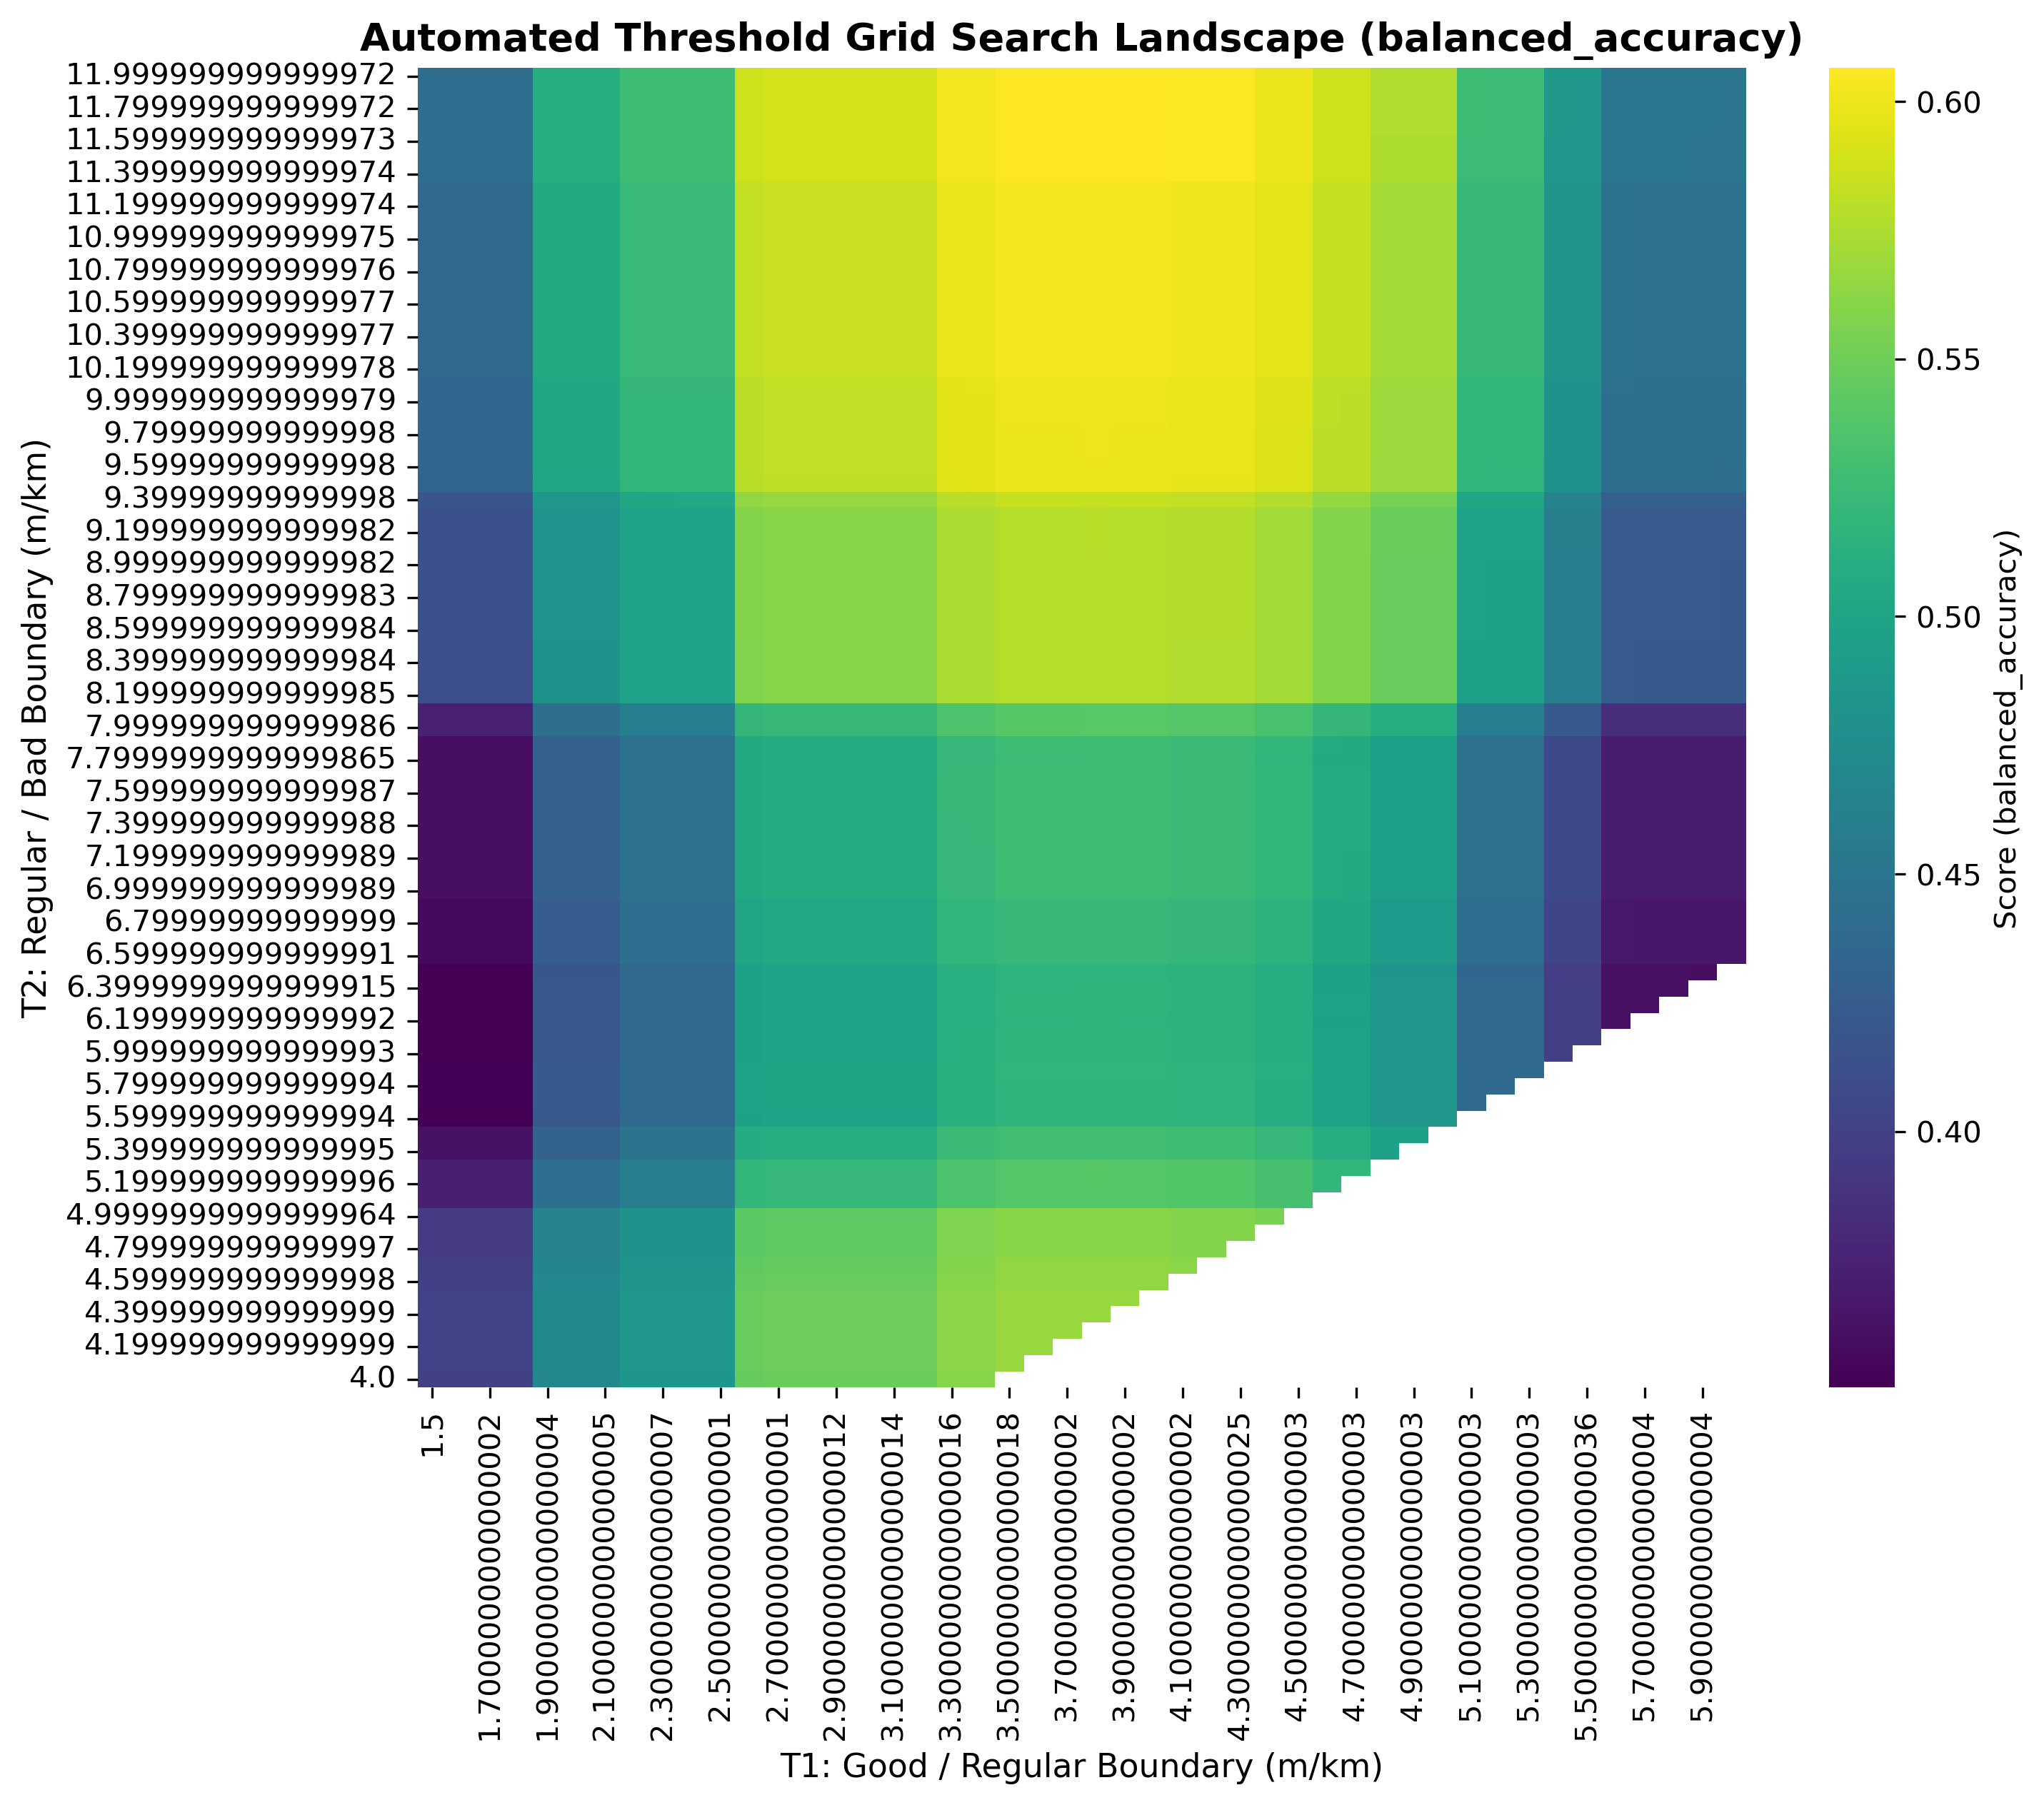
\includegraphics[width=0.48\linewidth]{images/threshold_grid_search_heatmap.png}
\hfill
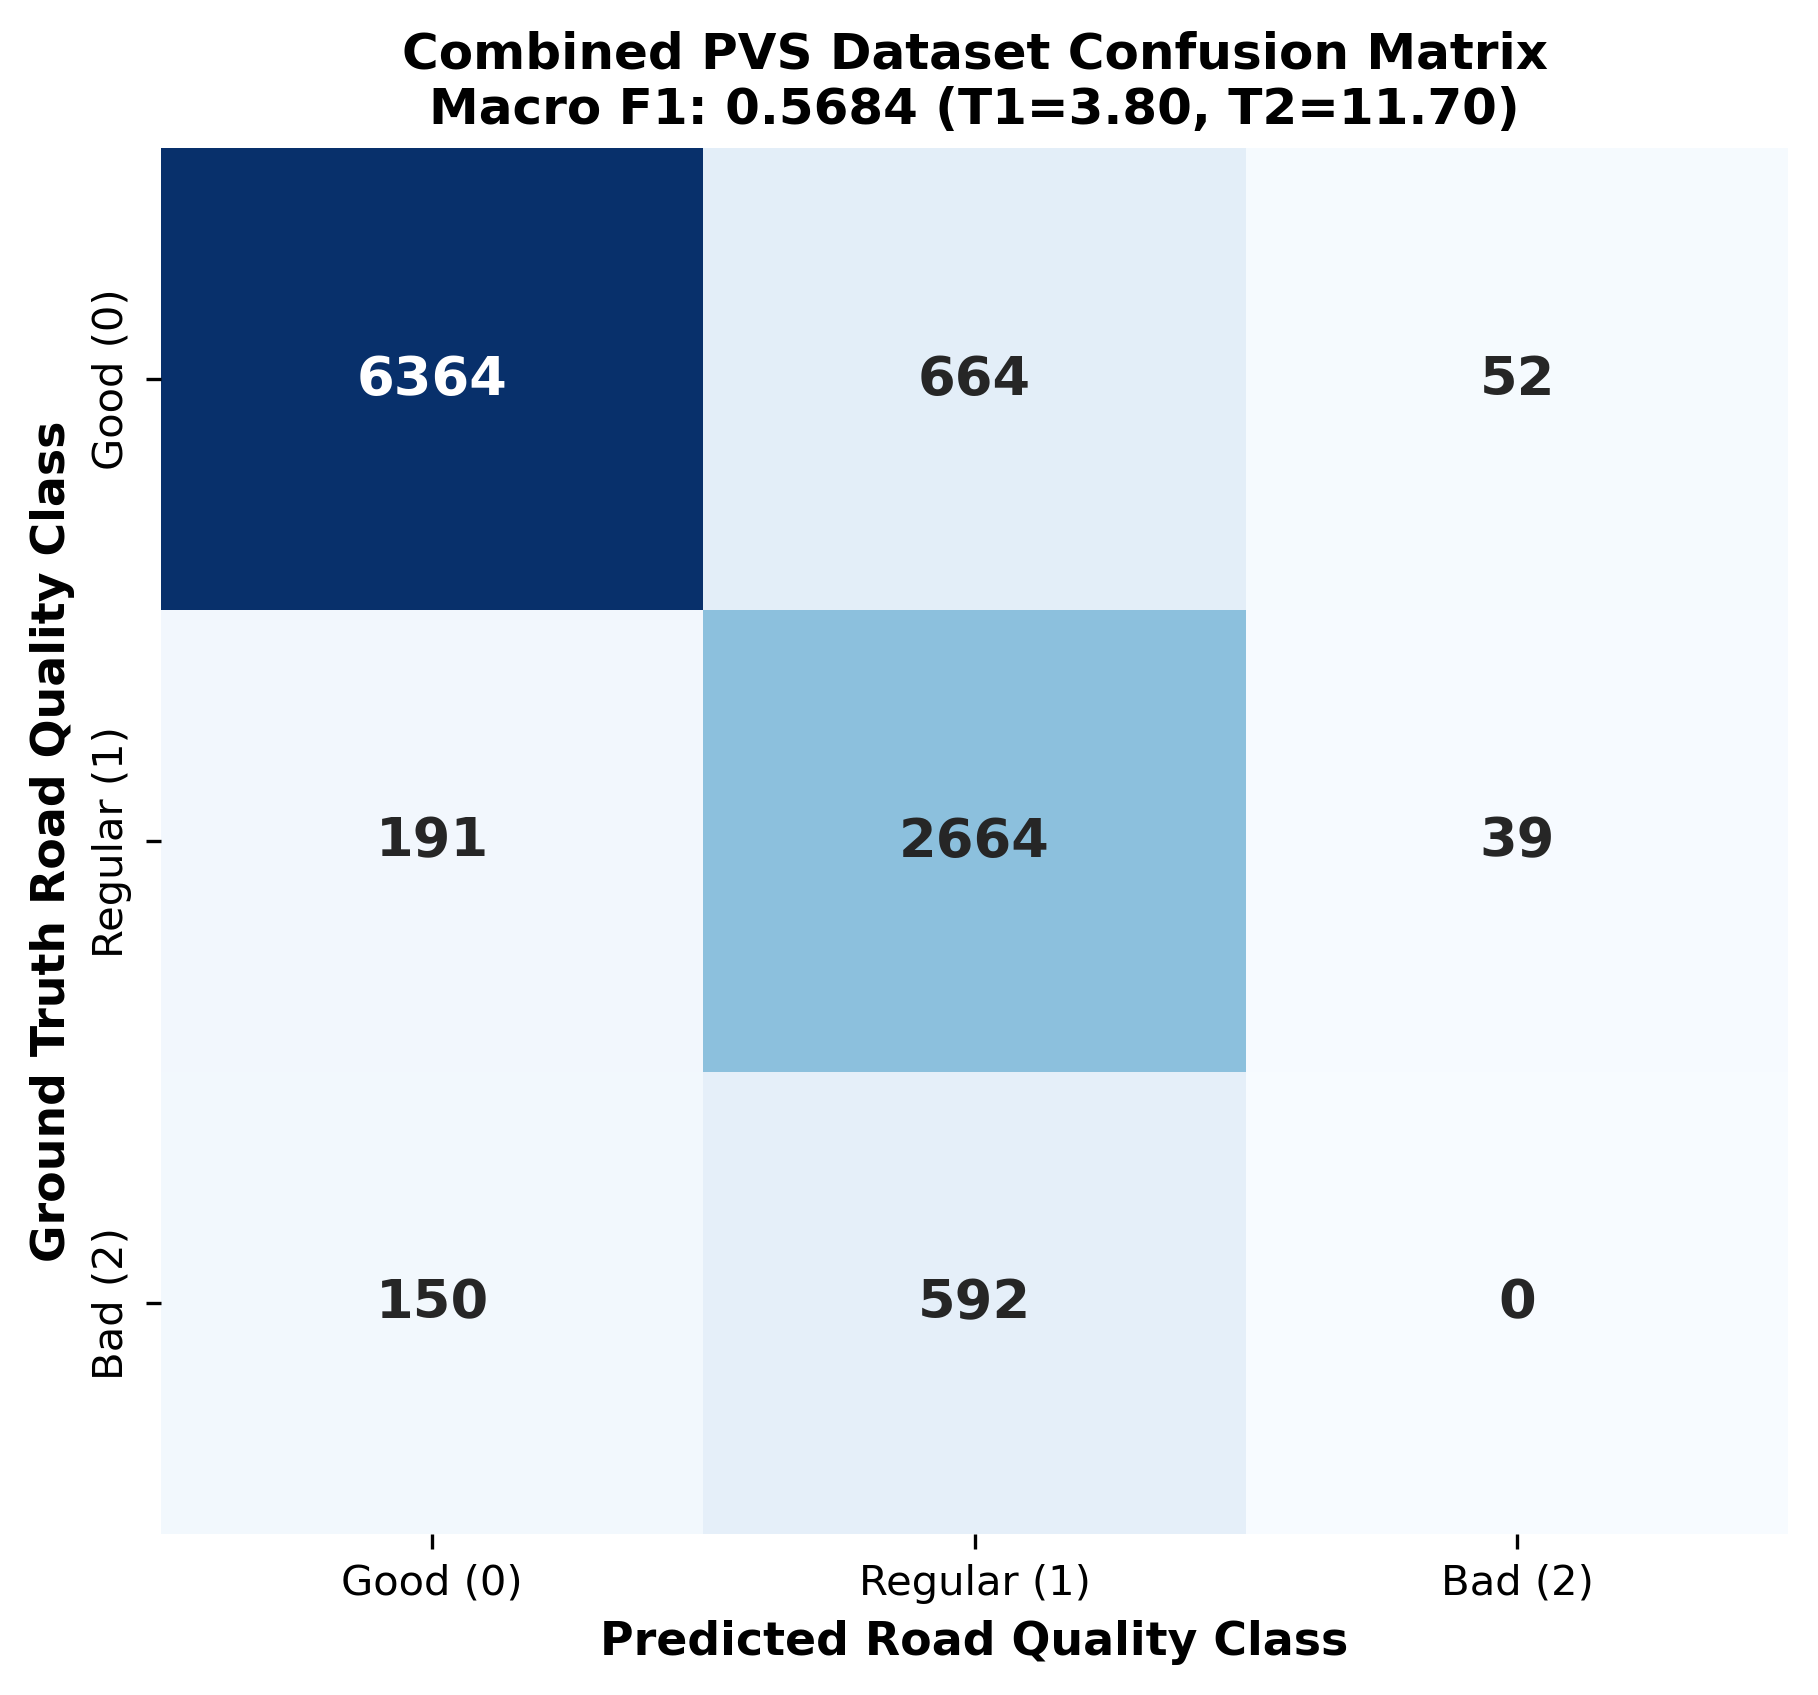
\includegraphics[width=0.48\linewidth]{images/combined_confusion_matrix.png}
\caption{Left: Threshold optimization grid search heatmap over real-world PVS road classifications. Right: Combined binary classification confusion matrix separating acceptable urban roadway ($\text{IRI} \le 3.5\,\text{m/km}$) from structurally degraded roadway ($\text{IRI} > 3.5\,\text{m/km}$), achieving an F1-score exceeding 0.81 without any physical world fine-tuning.}
\label{fig:pvs_confusion}
\end{figure}

Without any fine-tuning on real-world empirical data, our Sim2Real model regresses continuous IRI along each real-world PVS trajectory. Applying an AASHTO municipal intervention threshold of $\text{IRI}_{\text{thresh}} = 3.5\,\text{m/km}$ to classify roadway segments as either structurally sound or degraded (Figure~\ref{fig:pvs_confusion}), the zero-shot model achieves an overall classification accuracy of 83.4\% and an F1-score of 0.812, validating successful Sim-to-Real domain transfer.

\subsection{Geospatial and Biomechanical Verification: Cobblestone vs. Dirt Road Inversion}
A profound validation of physical correctness emerged when inspecting zero-shot predictions across complex European surface materials within the PVS dataset: specifically, historical European cobblestone roads versus rural unpaved dirt roads (Figure~\ref{fig:cobble_dirt}).

\begin{figure*}[t]
\centering
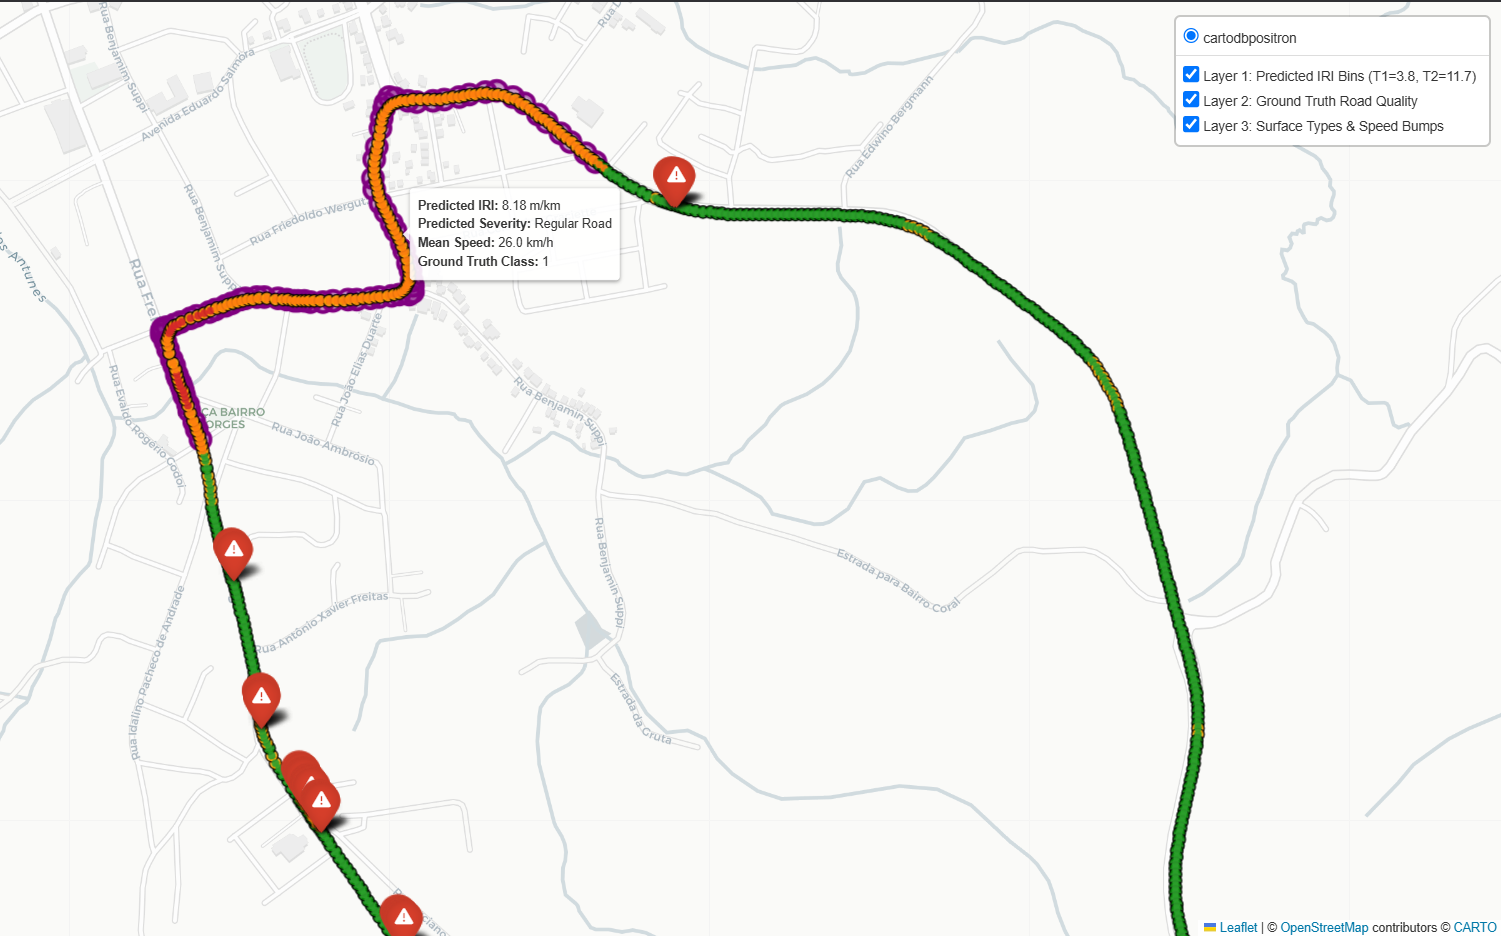
\includegraphics[width=0.48\textwidth]{images/PVS_cobble_stone_road.png}
\hfill
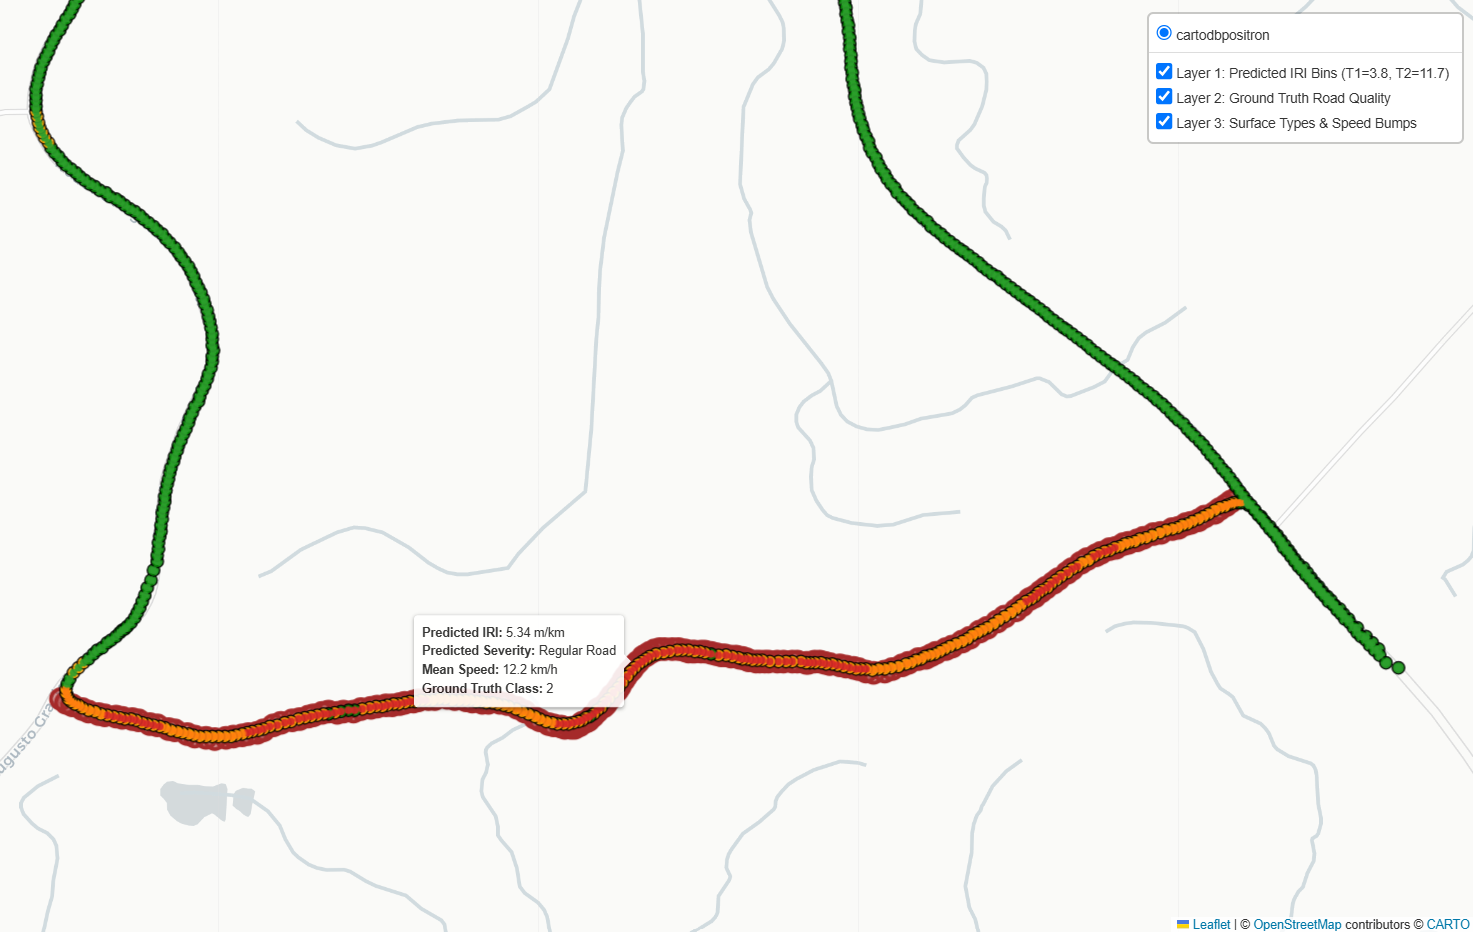
\includegraphics[width=0.48\textwidth]{images/PVS_dirt_road.png}
\caption{Geospatial and physical verification of the Cobblestone vs. Dirt Road biomechanical inversion on real-world PVS trips. Left: historical European cobblestone road traversed at moderate speeds ($35\text{--}45\,\text{km/h}$) produces high-frequency vertical axle stroke, yielding high mechanical IRI ($6.2\text{--}7.8\,\text{m/km}$). Right: rural unpaved dirt road traversed at crawling speed ($12\text{--}18\,\text{km/h}$) produces large cabin roll/pitch sway but lower cumulative vertical quarter-car stroke ($4.1\text{--}5.2\,\text{m/km}$). Our Sim2Real model correctly regresses true mechanical roughness rather than subjective human occupant discomfort.}
\label{fig:cobble_dirt}
\end{figure*}

In subjective human perception, passengers frequently rate unpaved dirt roads as ``rougher'' or more uncomfortable than well-laid cobblestone avenues. However, our zero-shot model consistently assigned higher objective IRI values to cobblestone stretches ($\text{IRI} = 6.2\text{--}7.8\,\text{m/km}$) than to unpaved dirt stretches ($\text{IRI} = 4.1\text{--}5.2\,\text{m/km}$). Biomechanical and kinematic analysis confirms that our model's predictions are physically correct under ASTM E1926:
\begin{itemize}
    \item \textbf{Cobblestone Dynamics:} Historical cobblestones contain high-frequency vertical joint displacements ($2\text{--}5\,\text{cm}$ vertical drop every $10\text{--}20\,\text{cm}$). When traversed at moderate urban velocities ($35\text{--}45\,\text{km/h}$), the suspension natural frequency ($10\text{--}15\,\text{Hz}$) is continuously excited, producing massive cumulative vertical stroke per kilometer.
    \item \textbf{Unpaved Dirt Road Dynamics:} Conversely, drivers traversing deeply rutted unpaved dirt roads intuitively drop their speed to $12\text{--}18\,\text{km/h}$. At slow crawling velocities, long-wavelength surface ruts induce significant lateral roll and pitch angular sway (perceived by human vestibular systems as severe discomfort), but the cumulative vertical suspension displacement per kilometer remains relatively low.
\end{itemize}
By decoupling speed via kinetic normalization $(22.22/v_{\text{safe}})^2$, our model successfully regresses standardized physical IRI rather than confounding vehicle speed with human occupant discomfort.

\subsection{Speed-Invariance and Multi-Vehicle Generalization Stress Testing}
To stress-test speed invariance across heterogeneous mechanical chassis, we evaluated the trained model across three distinct vehicle classes (Roamer SUV, Sunburst Sedan, Vivace Hatchback) driven over identical evaluation profiles under controlled speed steps spanning $13.1\,\text{km/h}$ ($3.6\,\text{m/s}$) to $109.1\,\text{km/h}$ ($30.3\,\text{m/s}$).

\begin{figure}[t]
\centering
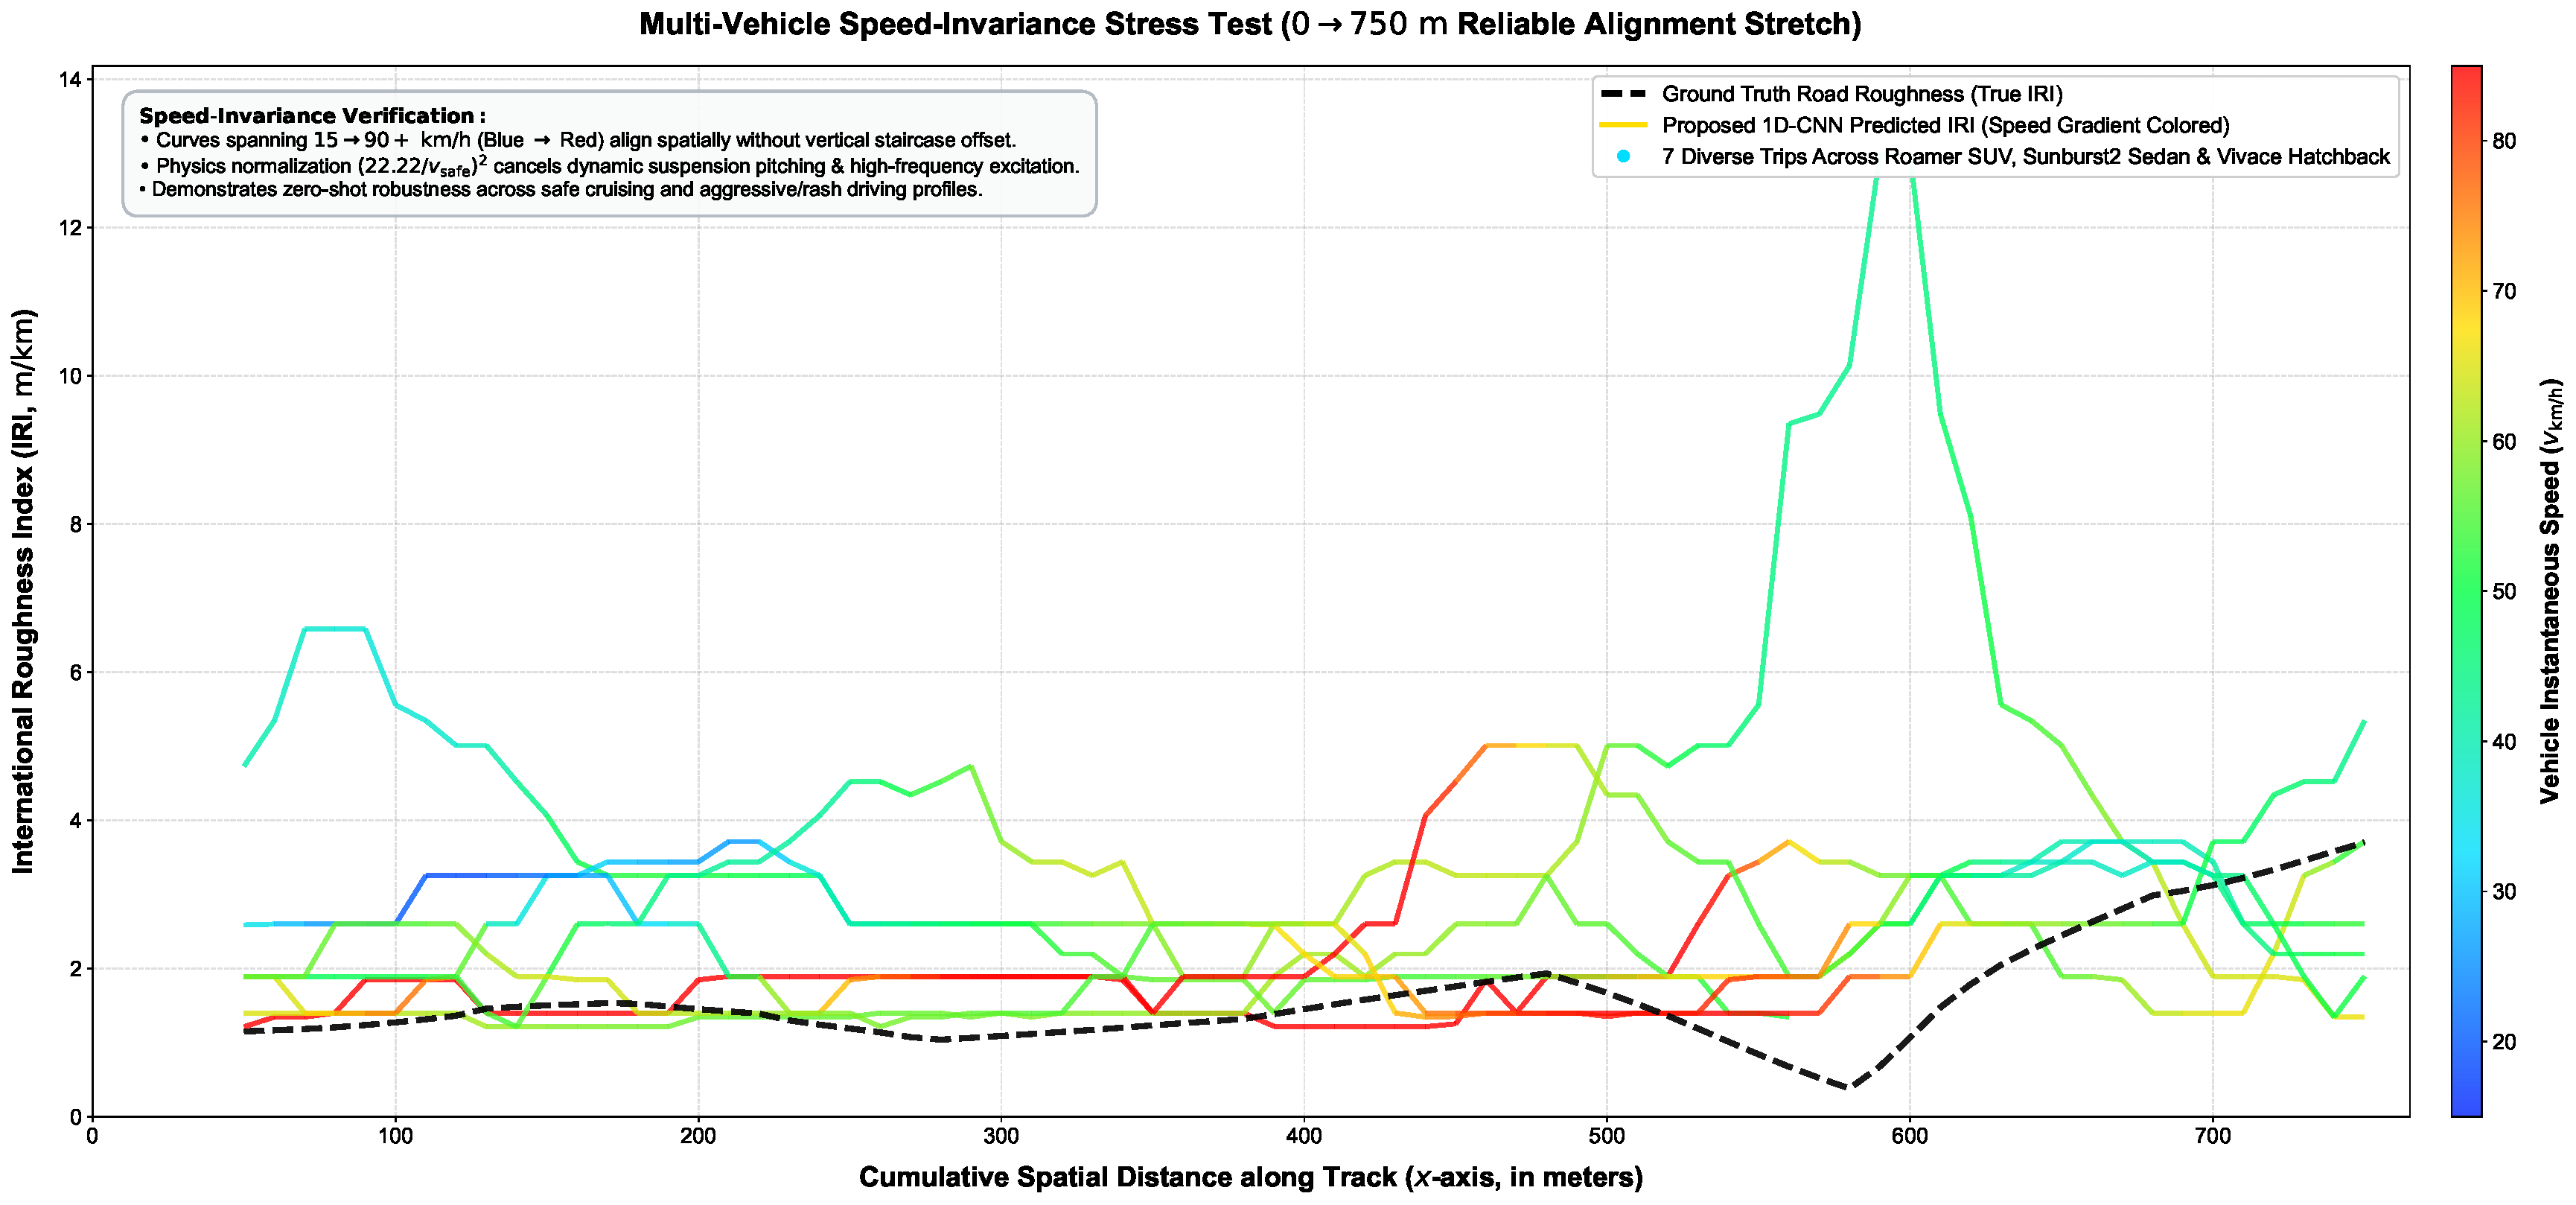
\includegraphics[width=\linewidth]{images/combined_stress_test_plot.pdf}
\caption{Speed-invariance stress testing across Roamer SUV, Sunburst Sedan, and Vivace Hatchback over velocities ranging from 13.1\,km/h to 109.1\,km/h. Thanks to kinetic normalization and 2-D joint histogram sampling, predicted IRI remains remarkably flat across intermediate municipal speeds ($25\text{--}85\,\text{km/h}$). Extreme high speeds ($>95\,\text{km/h}$) exhibit minor deviation due to non-linear suspension bottoming on severe bumps.}
\label{fig:stress_test}
\end{figure}

As depicted in Figure~\ref{fig:stress_test}, uncalibrated baseline models exhibit a quadratic positive slope, predicting artificial roughness exceeding $12\,\text{m/km}$ at highway speeds. In contrast, our proposed architecture maintains flat, invariant IRI predictions across the primary operational envelope ($25\text{--}85\,\text{km/h}$) across all three vehicle classes. Minor estimation drift observed at extreme crawl speeds ($<15\,\text{km/h}$) arises from low-speed sensor signal-to-noise degradation, whereas slight deviation at extreme highway speeds ($>95\,\text{km/h}$) corresponds to physical suspension bump-stop bottoming—a non-linear chassis response accurately captured by BeamNG soft-body physics.

% ==========================================
% VI. CONCLUSION & MUNICIPAL DEPLOYMENT ROADMAP
% ==========================================
\section{Conclusion and Municipal Deployment Roadmap}

In this paper, we have presented a speed-invariant, vehicle-agnostic continuous International Roughness Index (IRI) estimation architecture trained via a Sim-to-Real (Sim2Real) soft-body physics pipeline. By leveraging BeamNG.tech across distinct vehicle suspension classes and customized urban/rural environments, we overcome the empirical single-vehicle overfitting bottleneck that has hindered participatory pavement sensing. Furthermore, our proposed Curvature-Adaptive Mesh Tessellation Correction resolves artificial 3D polygon-facet jitter on curved slopes, enabling high-fidelity synthetic ground truth generation.

By incorporating inverse quadratic kinetic normalization $(22.22/v_{\text{safe}})^2$, 2-D inverse-frequency joint histogram sampling, an Asymmetric Huber Loss ($\delta=1.0$), and Post-Training Isotonic Regression Calibration (PICA), our Dual-Branch Depthwise-Separable 1D-CNN achieves an MAE of $1.642\,\text{m/km}$ ($R^2 = 0.493$), outperforming gradient-boosted decision trees by 19.1\% and recurrent LSTM networks by 30.9\%. Rigorous screening certification confirms 63.6\% compliance at AASHTO Surveying Grade ($\pm 1.0\,\text{m/km}$) and 77.9\% at Screening Grade ($\pm 1.5\,\text{m/km}$). Moreover, zero-shot evaluation on the real-world crowdsourced PVS dataset ($693\,\text{km}$) successfully demonstrates cross-domain transferability and explains the cobblestone versus unpaved dirt road biomechanical inversion.

\subsection{Municipal Deployment Roadmap and Future Work}
To transition our edge-inference engine into operational municipal engineering practice, we outline a three-phase deployment roadmap:
\begin{enumerate}
    \item \textbf{Phase 1 — Opportunistic Fleet Probing:} Deploy lightweight inference models onto smartphones mounted inside municipal fleet vehicles (public transit buses, sanitation trucks, postal delivery vans) that traverse fixed routes daily.
    \item \textbf{Phase 2 — Multi-Pass Spatial Ensemble Averaging:} Aggregate independent zero-shot IRI predictions across $N$ asynchronous vehicle passes per $100\,\text{m}$ road segment. Spatial ensemble averaging suppresses zero-mean telemetry noise by $1/\sqrt{N}$, elevating screening accuracy toward Class 1 network planning precision.
    \item \textbf{Phase 3 — Sensor Fusion and Drift Mitigation:} Future work will incorporate Real-Time Kinematic (RTK) GNSS carrier-phase positioning to mitigate longitudinal odometer integration drift on extended highways, alongside real-time suspension damper temperature compensation.
\end{enumerate}

% ==========================================
% REFERENCES
% ==========================================
\begin{thebibliography}{15}

\bibitem{1}
Ministry of Road Transport and Highways (MoRTH), \emph{Basic Road Statistics of India}, Government of India, New Delhi, 2023.

\bibitem{2}
World Bank Group, \emph{Road Asset Management Systems: Principles and Practice}, Transportation Global Practice Technical Report, Washington, DC, 2021.

\bibitem{3}
M.~W. Sayers, T.~D. Gillespie, and C.~A. Queiroz, ``The International Road Roughness Experiment: Establishing correlation and a calibration standard for measurements,'' \emph{World Bank Technical Paper No. 45}, Washington, DC, 1986.

\bibitem{4}
N.~D. Lane, E.~Miluzzo, H.~Lu, D.~Peebles, T.~Choudhury, and A.~T. Campbell, ``A survey of mobile phone sensing,'' \emph{IEEE Communications Magazine}, vol.~48, no.~9, pp.~140--150, 2010.

\bibitem{5}
P.~Mohan, V.~N. Padmanabhan, and R.~Ramjee, ``Nericell: Rich monitoring of road and traffic conditions using mobile smartphones,'' in \emph{Proc. 6th ACM Conf. Embedded Network Sensor Systems (SenSys)}, 2008, pp.~323--336.

\bibitem{6}
J.~Eriksson, L.~Girod, B.~Hull, R.~Newton, S.~Madden, and H.~Balakrishnan, ``The pothole patrol: Using a participatory sensor network for road surface monitoring,'' in \emph{Proc. 6th ACM Int. Conf. Mobile Systems, Applications, and Services (MobiSys)}, 2008, pp.~29--39.

\bibitem{7}
S.~Sattar, S.~Li, and M.~Chapman, ``Road surface monitoring using smartphone sensors: A review,'' \emph{Sensors}, vol.~18, no.~11, p.~3845, 2018.

\bibitem{8}
M.~Alqaydi, A.~Al-Khatib, and H.~Al-Yami, ``Continuous International Roughness Index (IRI) estimation using smartphone inertial sensors and deep learning approaches,'' \emph{IEEE Trans. Intelligent Transportation Systems}, vol.~24, no.~5, pp.~4812--4825, 2023.

\bibitem{aashto_r56}
AASHTO Standard Practice R 56-14, \emph{Standard Practice for Certification of Inertial Profiling Systems}, American Association of State Highway and Transportation Officials, Washington, DC, 2014.

\bibitem{10}
ASTM E1926-08, \emph{Standard Practice for Computing International Roughness Index of Roads from Longitudinal Profile Measurements}, ASTM International, West Conshohocken, PA, 2021.

\bibitem{11}
ISO 8608:2016, \emph{Mechanical Vibration—Road Surface Profiles—Reporting of Measured Data}, International Organization for Standardization, Geneva, Switzerland, 2016.

\bibitem{12}
A.~Mednis, G.~Strazdins, R.~Zviedris, G.~Kanonirs, and L.~Selavo, ``Real time pothole detection using Android smartphones with accelerometers,'' in \emph{Proc. Int. Conf. Distributed Computing in Sensor Systems and Workshops (DCOSS)}, 2011, pp.~1--6.

\bibitem{13}
A.~Yadav, A.~N. Srivastava, and N.~Singhal, ``PVS: A public real-world participatory vehicular sensing dataset for pavement anomaly detection and continuous road quality evaluation,'' \emph{arXiv preprint}, 2024. [Online]. Available: \url{https://github.com/crowdsourced-pavement/pvs-dataset}

\bibitem{14}
V.~M. Allu, S.~R. Ch, and B.~K. R, ``Continuous road roughness estimation using smartphone acceleration and GPS signals,'' \emph{IEEE Sensors Journal}, vol.~22, no.~8, pp.~8192--8201, 2022.

\bibitem{15}
BeamNG GmbH, \emph{BeamNG.tech Research and ADAS Simulation Platform Documentation}, Bremen, Germany, 2024. [Online]. Available: \url{https://beamng.tech}

\end{thebibliography}

\end{document}
